\documentclass{article}


% if you need to pass options to natbib, use, e.g.:
%     \PassOptionsToPackage{numbers, compress}{natbib}
% before loading neurips_2024


\usepackage[utf8]{inputenc} % allow utf-8 input
\usepackage[T1]{fontenc}    % use 8-bit T1 fonts
\usepackage{hyperref}       % hyperlinks
\usepackage{url}            % simple URL typesetting
\usepackage{booktabs}       % professional-quality tables
\usepackage{amsfonts}       % blackboard math symbols
\usepackage{nicefrac}       % compact symbols for 1/2, etc.
\usepackage{microtype}      % microtypography
\usepackage{xcolor}         % colors


\usepackage{graphicx}
%\usepackage{subfigure}
\usepackage{caption}
\usepackage{subcaption}
\usepackage{booktabs}
\usepackage{tikz}
\usetikzlibrary{shapes.multipart}
\usetikzlibrary{calc}
\usetikzlibrary{backgrounds}


\usepackage{latexsym}
\usepackage{tabularx}
\usepackage{multirow}
\usepackage{enumitem}
\usepackage{amsmath}
\usepackage{pifont}
\usepackage{amssymb}
\usepackage{color, colortbl}
\usepackage{float}
\usepackage{dblfloatfix}
\usepackage{appendix}
\usepackage{bbold}
\usepackage{xspace}
\usepackage{adjustbox}
\usepackage{changepage}
%%%%% NEW MATH DEFINITIONS %%%%%

\usepackage{amsmath,amsfonts,bm}
\usepackage{derivative}
% Mark sections of captions for referring to divisions of figures
\newcommand{\figleft}{{\em (Left)}}
\newcommand{\figcenter}{{\em (Center)}}
\newcommand{\figright}{{\em (Right)}}
\newcommand{\figtop}{{\em (Top)}}
\newcommand{\figbottom}{{\em (Bottom)}}
\newcommand{\captiona}{{\em (a)}}
\newcommand{\captionb}{{\em (b)}}
\newcommand{\captionc}{{\em (c)}}
\newcommand{\captiond}{{\em (d)}}

% Highlight a newly defined term
\newcommand{\newterm}[1]{{\bf #1}}

% Derivative d 
\newcommand{\deriv}{{\mathrm{d}}}

% Figure reference, lower-case.
\def\figref#1{figure~\ref{#1}}
% Figure reference, capital. For start of sentence
\def\Figref#1{Figure~\ref{#1}}
\def\twofigref#1#2{figures \ref{#1} and \ref{#2}}
\def\quadfigref#1#2#3#4{figures \ref{#1}, \ref{#2}, \ref{#3} and \ref{#4}}
% Section reference, lower-case.
\def\secref#1{section~\ref{#1}}
% Section reference, capital.
\def\Secref#1{Section~\ref{#1}}
% Reference to two sections.
\def\twosecrefs#1#2{sections \ref{#1} and \ref{#2}}
% Reference to three sections.
\def\secrefs#1#2#3{sections \ref{#1}, \ref{#2} and \ref{#3}}
% Reference to an equation, lower-case.
\def\eqref#1{equation~\ref{#1}}
% Reference to an equation, upper case
\def\Eqref#1{Equation~\ref{#1}}
% A raw reference to an equation---avoid using if possible
\def\plaineqref#1{\ref{#1}}
% Reference to a chapter, lower-case.
\def\chapref#1{chapter~\ref{#1}}
% Reference to an equation, upper case.
\def\Chapref#1{Chapter~\ref{#1}}
% Reference to a range of chapters
\def\rangechapref#1#2{chapters\ref{#1}--\ref{#2}}
% Reference to an algorithm, lower-case.
\def\algref#1{algorithm~\ref{#1}}
% Reference to an algorithm, upper case.
\def\Algref#1{Algorithm~\ref{#1}}
\def\twoalgref#1#2{algorithms \ref{#1} and \ref{#2}}
\def\Twoalgref#1#2{Algorithms \ref{#1} and \ref{#2}}
% Reference to a part, lower case
\def\partref#1{part~\ref{#1}}
% Reference to a part, upper case
\def\Partref#1{Part~\ref{#1}}
\def\twopartref#1#2{parts \ref{#1} and \ref{#2}}

\def\ceil#1{\lceil #1 \rceil}
\def\floor#1{\lfloor #1 \rfloor}
\def\1{\bm{1}}
\newcommand{\train}{\mathcal{D}}
\newcommand{\valid}{\mathcal{D_{\mathrm{valid}}}}
\newcommand{\test}{\mathcal{D_{\mathrm{test}}}}

\def\eps{{\epsilon}}


% Random variables
\def\reta{{\textnormal{$\eta$}}}
\def\ra{{\textnormal{a}}}
\def\rb{{\textnormal{b}}}
\def\rc{{\textnormal{c}}}
\def\rd{{\textnormal{d}}}
\def\re{{\textnormal{e}}}
\def\rf{{\textnormal{f}}}
\def\rg{{\textnormal{g}}}
\def\rh{{\textnormal{h}}}
\def\ri{{\textnormal{i}}}
\def\rj{{\textnormal{j}}}
\def\rk{{\textnormal{k}}}
\def\rl{{\textnormal{l}}}
% rm is already a command, just don't name any random variables m
\def\rn{{\textnormal{n}}}
\def\ro{{\textnormal{o}}}
\def\rp{{\textnormal{p}}}
\def\rq{{\textnormal{q}}}
\def\rr{{\textnormal{r}}}
\def\rs{{\textnormal{s}}}
\def\rt{{\textnormal{t}}}
\def\ru{{\textnormal{u}}}
\def\rv{{\textnormal{v}}}
\def\rw{{\textnormal{w}}}
\def\rx{{\textnormal{x}}}
\def\ry{{\textnormal{y}}}
\def\rz{{\textnormal{z}}}

% Random vectors
\def\rvepsilon{{\mathbf{\epsilon}}}
\def\rvphi{{\mathbf{\phi}}}
\def\rvtheta{{\mathbf{\theta}}}
\def\rva{{\mathbf{a}}}
\def\rvb{{\mathbf{b}}}
\def\rvc{{\mathbf{c}}}
\def\rvd{{\mathbf{d}}}
\def\rve{{\mathbf{e}}}
\def\rvf{{\mathbf{f}}}
\def\rvg{{\mathbf{g}}}
\def\rvh{{\mathbf{h}}}
\def\rvu{{\mathbf{i}}}
\def\rvj{{\mathbf{j}}}
\def\rvk{{\mathbf{k}}}
\def\rvl{{\mathbf{l}}}
\def\rvm{{\mathbf{m}}}
\def\rvn{{\mathbf{n}}}
\def\rvo{{\mathbf{o}}}
\def\rvp{{\mathbf{p}}}
\def\rvq{{\mathbf{q}}}
\def\rvr{{\mathbf{r}}}
\def\rvs{{\mathbf{s}}}
\def\rvt{{\mathbf{t}}}
\def\rvu{{\mathbf{u}}}
\def\rvv{{\mathbf{v}}}
\def\rvw{{\mathbf{w}}}
\def\rvx{{\mathbf{x}}}
\def\rvy{{\mathbf{y}}}
\def\rvz{{\mathbf{z}}}

% Elements of random vectors
\def\erva{{\textnormal{a}}}
\def\ervb{{\textnormal{b}}}
\def\ervc{{\textnormal{c}}}
\def\ervd{{\textnormal{d}}}
\def\erve{{\textnormal{e}}}
\def\ervf{{\textnormal{f}}}
\def\ervg{{\textnormal{g}}}
\def\ervh{{\textnormal{h}}}
\def\ervi{{\textnormal{i}}}
\def\ervj{{\textnormal{j}}}
\def\ervk{{\textnormal{k}}}
\def\ervl{{\textnormal{l}}}
\def\ervm{{\textnormal{m}}}
\def\ervn{{\textnormal{n}}}
\def\ervo{{\textnormal{o}}}
\def\ervp{{\textnormal{p}}}
\def\ervq{{\textnormal{q}}}
\def\ervr{{\textnormal{r}}}
\def\ervs{{\textnormal{s}}}
\def\ervt{{\textnormal{t}}}
\def\ervu{{\textnormal{u}}}
\def\ervv{{\textnormal{v}}}
\def\ervw{{\textnormal{w}}}
\def\ervx{{\textnormal{x}}}
\def\ervy{{\textnormal{y}}}
\def\ervz{{\textnormal{z}}}

% Random matrices
\def\rmA{{\mathbf{A}}}
\def\rmB{{\mathbf{B}}}
\def\rmC{{\mathbf{C}}}
\def\rmD{{\mathbf{D}}}
\def\rmE{{\mathbf{E}}}
\def\rmF{{\mathbf{F}}}
\def\rmG{{\mathbf{G}}}
\def\rmH{{\mathbf{H}}}
\def\rmI{{\mathbf{I}}}
\def\rmJ{{\mathbf{J}}}
\def\rmK{{\mathbf{K}}}
\def\rmL{{\mathbf{L}}}
\def\rmM{{\mathbf{M}}}
\def\rmN{{\mathbf{N}}}
\def\rmO{{\mathbf{O}}}
\def\rmP{{\mathbf{P}}}
\def\rmQ{{\mathbf{Q}}}
\def\rmR{{\mathbf{R}}}
\def\rmS{{\mathbf{S}}}
\def\rmT{{\mathbf{T}}}
\def\rmU{{\mathbf{U}}}
\def\rmV{{\mathbf{V}}}
\def\rmW{{\mathbf{W}}}
\def\rmX{{\mathbf{X}}}
\def\rmY{{\mathbf{Y}}}
\def\rmZ{{\mathbf{Z}}}

% Elements of random matrices
\def\ermA{{\textnormal{A}}}
\def\ermB{{\textnormal{B}}}
\def\ermC{{\textnormal{C}}}
\def\ermD{{\textnormal{D}}}
\def\ermE{{\textnormal{E}}}
\def\ermF{{\textnormal{F}}}
\def\ermG{{\textnormal{G}}}
\def\ermH{{\textnormal{H}}}
\def\ermI{{\textnormal{I}}}
\def\ermJ{{\textnormal{J}}}
\def\ermK{{\textnormal{K}}}
\def\ermL{{\textnormal{L}}}
\def\ermM{{\textnormal{M}}}
\def\ermN{{\textnormal{N}}}
\def\ermO{{\textnormal{O}}}
\def\ermP{{\textnormal{P}}}
\def\ermQ{{\textnormal{Q}}}
\def\ermR{{\textnormal{R}}}
\def\ermS{{\textnormal{S}}}
\def\ermT{{\textnormal{T}}}
\def\ermU{{\textnormal{U}}}
\def\ermV{{\textnormal{V}}}
\def\ermW{{\textnormal{W}}}
\def\ermX{{\textnormal{X}}}
\def\ermY{{\textnormal{Y}}}
\def\ermZ{{\textnormal{Z}}}

% Vectors
\def\vzero{{\bm{0}}}
\def\vone{{\bm{1}}}
\def\vmu{{\bm{\mu}}}
\def\vtheta{{\bm{\theta}}}
\def\vphi{{\bm{\phi}}}
\def\va{{\bm{a}}}
\def\vb{{\bm{b}}}
\def\vc{{\bm{c}}}
\def\vd{{\bm{d}}}
\def\ve{{\bm{e}}}
\def\vf{{\bm{f}}}
\def\vg{{\bm{g}}}
\def\vh{{\bm{h}}}
\def\vi{{\bm{i}}}
\def\vj{{\bm{j}}}
\def\vk{{\bm{k}}}
\def\vl{{\bm{l}}}
\def\vm{{\bm{m}}}
\def\vn{{\bm{n}}}
\def\vo{{\bm{o}}}
\def\vp{{\bm{p}}}
\def\vq{{\bm{q}}}
\def\vr{{\bm{r}}}
\def\vs{{\bm{s}}}
\def\vt{{\bm{t}}}
\def\vu{{\bm{u}}}
\def\vv{{\bm{v}}}
\def\vw{{\bm{w}}}
\def\vx{{\bm{x}}}
\def\vy{{\bm{y}}}
\def\vz{{\bm{z}}}

% Elements of vectors
\def\evalpha{{\alpha}}
\def\evbeta{{\beta}}
\def\evepsilon{{\epsilon}}
\def\evlambda{{\lambda}}
\def\evomega{{\omega}}
\def\evmu{{\mu}}
\def\evpsi{{\psi}}
\def\evsigma{{\sigma}}
\def\evtheta{{\theta}}
\def\eva{{a}}
\def\evb{{b}}
\def\evc{{c}}
\def\evd{{d}}
\def\eve{{e}}
\def\evf{{f}}
\def\evg{{g}}
\def\evh{{h}}
\def\evi{{i}}
\def\evj{{j}}
\def\evk{{k}}
\def\evl{{l}}
\def\evm{{m}}
\def\evn{{n}}
\def\evo{{o}}
\def\evp{{p}}
\def\evq{{q}}
\def\evr{{r}}
\def\evs{{s}}
\def\evt{{t}}
\def\evu{{u}}
\def\evv{{v}}
\def\evw{{w}}
\def\evx{{x}}
\def\evy{{y}}
\def\evz{{z}}

% Matrix
\def\mA{{\bm{A}}}
\def\mB{{\bm{B}}}
\def\mC{{\bm{C}}}
\def\mD{{\bm{D}}}
\def\mE{{\bm{E}}}
\def\mF{{\bm{F}}}
\def\mG{{\bm{G}}}
\def\mH{{\bm{H}}}
\def\mI{{\bm{I}}}
\def\mJ{{\bm{J}}}
\def\mK{{\bm{K}}}
\def\mL{{\bm{L}}}
\def\mM{{\bm{M}}}
\def\mN{{\bm{N}}}
\def\mO{{\bm{O}}}
\def\mP{{\bm{P}}}
\def\mQ{{\bm{Q}}}
\def\mR{{\bm{R}}}
\def\mS{{\bm{S}}}
\def\mT{{\bm{T}}}
\def\mU{{\bm{U}}}
\def\mV{{\bm{V}}}
\def\mW{{\bm{W}}}
\def\mX{{\bm{X}}}
\def\mY{{\bm{Y}}}
\def\mZ{{\bm{Z}}}
\def\mBeta{{\bm{\beta}}}
\def\mPhi{{\bm{\Phi}}}
\def\mLambda{{\bm{\Lambda}}}
\def\mSigma{{\bm{\Sigma}}}

% Tensor
\DeclareMathAlphabet{\mathsfit}{\encodingdefault}{\sfdefault}{m}{sl}
\SetMathAlphabet{\mathsfit}{bold}{\encodingdefault}{\sfdefault}{bx}{n}
\newcommand{\tens}[1]{\bm{\mathsfit{#1}}}
\def\tA{{\tens{A}}}
\def\tB{{\tens{B}}}
\def\tC{{\tens{C}}}
\def\tD{{\tens{D}}}
\def\tE{{\tens{E}}}
\def\tF{{\tens{F}}}
\def\tG{{\tens{G}}}
\def\tH{{\tens{H}}}
\def\tI{{\tens{I}}}
\def\tJ{{\tens{J}}}
\def\tK{{\tens{K}}}
\def\tL{{\tens{L}}}
\def\tM{{\tens{M}}}
\def\tN{{\tens{N}}}
\def\tO{{\tens{O}}}
\def\tP{{\tens{P}}}
\def\tQ{{\tens{Q}}}
\def\tR{{\tens{R}}}
\def\tS{{\tens{S}}}
\def\tT{{\tens{T}}}
\def\tU{{\tens{U}}}
\def\tV{{\tens{V}}}
\def\tW{{\tens{W}}}
\def\tX{{\tens{X}}}
\def\tY{{\tens{Y}}}
\def\tZ{{\tens{Z}}}


% Graph
\def\gA{{\mathcal{A}}}
\def\gB{{\mathcal{B}}}
\def\gC{{\mathcal{C}}}
\def\gD{{\mathcal{D}}}
\def\gE{{\mathcal{E}}}
\def\gF{{\mathcal{F}}}
\def\gG{{\mathcal{G}}}
\def\gH{{\mathcal{H}}}
\def\gI{{\mathcal{I}}}
\def\gJ{{\mathcal{J}}}
\def\gK{{\mathcal{K}}}
\def\gL{{\mathcal{L}}}
\def\gM{{\mathcal{M}}}
\def\gN{{\mathcal{N}}}
\def\gO{{\mathcal{O}}}
\def\gP{{\mathcal{P}}}
\def\gQ{{\mathcal{Q}}}
\def\gR{{\mathcal{R}}}
\def\gS{{\mathcal{S}}}
\def\gT{{\mathcal{T}}}
\def\gU{{\mathcal{U}}}
\def\gV{{\mathcal{V}}}
\def\gW{{\mathcal{W}}}
\def\gX{{\mathcal{X}}}
\def\gY{{\mathcal{Y}}}
\def\gZ{{\mathcal{Z}}}

% Sets
\def\sA{{\mathbb{A}}}
\def\sB{{\mathbb{B}}}
\def\sC{{\mathbb{C}}}
\def\sD{{\mathbb{D}}}
% Don't use a set called E, because this would be the same as our symbol
% for expectation.
\def\sF{{\mathbb{F}}}
\def\sG{{\mathbb{G}}}
\def\sH{{\mathbb{H}}}
\def\sI{{\mathbb{I}}}
\def\sJ{{\mathbb{J}}}
\def\sK{{\mathbb{K}}}
\def\sL{{\mathbb{L}}}
\def\sM{{\mathbb{M}}}
\def\sN{{\mathbb{N}}}
\def\sO{{\mathbb{O}}}
\def\sP{{\mathbb{P}}}
\def\sQ{{\mathbb{Q}}}
\def\sR{{\mathbb{R}}}
\def\sS{{\mathbb{S}}}
\def\sT{{\mathbb{T}}}
\def\sU{{\mathbb{U}}}
\def\sV{{\mathbb{V}}}
\def\sW{{\mathbb{W}}}
\def\sX{{\mathbb{X}}}
\def\sY{{\mathbb{Y}}}
\def\sZ{{\mathbb{Z}}}

% Entries of a matrix
\def\emLambda{{\Lambda}}
\def\emA{{A}}
\def\emB{{B}}
\def\emC{{C}}
\def\emD{{D}}
\def\emE{{E}}
\def\emF{{F}}
\def\emG{{G}}
\def\emH{{H}}
\def\emI{{I}}
\def\emJ{{J}}
\def\emK{{K}}
\def\emL{{L}}
\def\emM{{M}}
\def\emN{{N}}
\def\emO{{O}}
\def\emP{{P}}
\def\emQ{{Q}}
\def\emR{{R}}
\def\emS{{S}}
\def\emT{{T}}
\def\emU{{U}}
\def\emV{{V}}
\def\emW{{W}}
\def\emX{{X}}
\def\emY{{Y}}
\def\emZ{{Z}}
\def\emSigma{{\Sigma}}

% entries of a tensor
% Same font as tensor, without \bm wrapper
\newcommand{\etens}[1]{\mathsfit{#1}}
\def\etLambda{{\etens{\Lambda}}}
\def\etA{{\etens{A}}}
\def\etB{{\etens{B}}}
\def\etC{{\etens{C}}}
\def\etD{{\etens{D}}}
\def\etE{{\etens{E}}}
\def\etF{{\etens{F}}}
\def\etG{{\etens{G}}}
\def\etH{{\etens{H}}}
\def\etI{{\etens{I}}}
\def\etJ{{\etens{J}}}
\def\etK{{\etens{K}}}
\def\etL{{\etens{L}}}
\def\etM{{\etens{M}}}
\def\etN{{\etens{N}}}
\def\etO{{\etens{O}}}
\def\etP{{\etens{P}}}
\def\etQ{{\etens{Q}}}
\def\etR{{\etens{R}}}
\def\etS{{\etens{S}}}
\def\etT{{\etens{T}}}
\def\etU{{\etens{U}}}
\def\etV{{\etens{V}}}
\def\etW{{\etens{W}}}
\def\etX{{\etens{X}}}
\def\etY{{\etens{Y}}}
\def\etZ{{\etens{Z}}}

% The true underlying data generating distribution
\newcommand{\pdata}{p_{\rm{data}}}
\newcommand{\ptarget}{p_{\rm{target}}}
\newcommand{\pprior}{p_{\rm{prior}}}
\newcommand{\pbase}{p_{\rm{base}}}
\newcommand{\pref}{p_{\rm{ref}}}

% The empirical distribution defined by the training set
\newcommand{\ptrain}{\hat{p}_{\rm{data}}}
\newcommand{\Ptrain}{\hat{P}_{\rm{data}}}
% The model distribution
\newcommand{\pmodel}{p_{\rm{model}}}
\newcommand{\Pmodel}{P_{\rm{model}}}
\newcommand{\ptildemodel}{\tilde{p}_{\rm{model}}}
% Stochastic autoencoder distributions
\newcommand{\pencode}{p_{\rm{encoder}}}
\newcommand{\pdecode}{p_{\rm{decoder}}}
\newcommand{\precons}{p_{\rm{reconstruct}}}

\newcommand{\laplace}{\mathrm{Laplace}} % Laplace distribution

\newcommand{\E}{\mathbb{E}}
\newcommand{\Ls}{\mathcal{L}}
\newcommand{\R}{\mathbb{R}}
\newcommand{\emp}{\tilde{p}}
\newcommand{\lr}{\alpha}
\newcommand{\reg}{\lambda}
\newcommand{\rect}{\mathrm{rectifier}}
\newcommand{\softmax}{\mathrm{softmax}}
\newcommand{\sigmoid}{\sigma}
\newcommand{\softplus}{\zeta}
\newcommand{\KL}{D_{\mathrm{KL}}}
\newcommand{\Var}{\mathrm{Var}}
\newcommand{\standarderror}{\mathrm{SE}}
\newcommand{\Cov}{\mathrm{Cov}}
% Wolfram Mathworld says $L^2$ is for function spaces and $\ell^2$ is for vectors
% But then they seem to use $L^2$ for vectors throughout the site, and so does
% wikipedia.
\newcommand{\normlzero}{L^0}
\newcommand{\normlone}{L^1}
\newcommand{\normltwo}{L^2}
\newcommand{\normlp}{L^p}
\newcommand{\normmax}{L^\infty}

\newcommand{\parents}{Pa} % See usage in notation.tex. Chosen to match Daphne's book.

\DeclareMathOperator*{\argmax}{arg\,max}
\DeclareMathOperator*{\argmin}{arg\,min}

\DeclareMathOperator{\sign}{sign}
\DeclareMathOperator{\Tr}{Tr}
\let\ab\allowbreak

\definecolor{DarkPink}{rgb}{0.5,0.0,0.18}
\definecolor{DarkGreen}{rgb}{0.1,0.5,0.1}
\definecolor{DarkRed}{rgb}{0.5,0.1,0.1}
\definecolor{DarkBlue}{rgb}{0.1,0.1,0.7}
\definecolor{DarkYellow}{rgb}{.79,.79,0}
\hypersetup{
    unicode=false,          % non-Latin characters in Acrobat¿s bookmarks
    pdftoolbar=true,        % show Acrobat toolbar?
    pdfmenubar=true,        % show Acrobat menu?
    pdffitwindow=false,      % page fit to window when opened
    pdfnewwindow=true,      % links in new window
    colorlinks=true,       % false: boxed links; true: colored links
    linkcolor=DarkBlue,          % color of internal links
    citecolor=DarkPink,        % color of links to bibliography
    filecolor=DarkRed,      % color of file links
    urlcolor=DarkBlue,          % color of external links
    %
    % paper specific, please update
    %
    pdftitle={},
    pdfauthor={},
}

\usepackage[accepted]{icml2025}

% For theorems and such
\usepackage{amsmath}
\usepackage{amssymb}
\usepackage{mathtools}
\usepackage{amsthm}

\newcommand{\matteo}[1]{{\color{magenta}\{\textit{#1}\}$_{matteo}$}}


% to compile a preprint version, e.g., for submission to arXiv, add add the
% [preprint] option:
%     \usepackage[preprint]{neurips_2024}


% to compile a camera-ready version, add the [final] option, e.g.:
%     \usepackage[final]{neurips_2024}


% to avoid loading the natbib package, add option nonatbib:
%    \usepackage[nonatbib]{neurips_2024}

\icmltitlerunning{Leveraging the true depth of LLMs}


% \title{Leveraging the true depth of LLMs}


% The \author macro works with any number of authors. There are two commands
% used to separate the names and addresses of multiple authors: \And and \AND.
%
% Using \And between authors leaves it to LaTeX to determine where to break the
% lines. Using \AND forces a line break at that point. So, if LaTeX puts 3 of 4
% authors names on the first line, and the last on the second line, try using
% \AND instead of \And before the third author name.


%\author{%
%  David S.~Hippocampus\thanks{Use footnote for providing further information
%    about author (webpage, alternative address)---\emph{not} for acknowledging
%    funding agencies.} \\
%  Department of Computer Science\\
%  Cranberry-Lemon University\\
%  Pittsburgh, PA 15213 \\
%  \texttt{hippo@cs.cranberry-lemon.edu} \\
  % examples of more authors
  % \And
  % Coauthor \\
  % Affiliation \\
  % Address \\
  % \texttt{email} \\
  % \AND
  % Coauthor \\
  % Affiliation \\
  % Address \\
  % \texttt{email} \\
  % \And
  % Coauthor \\
  % Affiliation \\
  % Address \\
  % \texttt{email} \\
  % \And
  % Coauthor \\
  % Affiliation \\
  % Address \\
  % \texttt{email} \\
%}


\makeatletter
\def\mathcolor#1#{\@mathcolor{#1}}
\def\@mathcolor#1#2#3{%
  \protect\leavevmode
  \begingroup
    \color#1{#2}#3%
  \endgroup
}
\makeatother

% Define some common color schemes
\definecolor{feature1}{RGB}{230,230,250} % Lavender
\definecolor{feature2}{RGB}{176,224,230} % Powder blue
\definecolor{feature3}{RGB}{144,238,144} % Light green
\definecolor{feature4}{RGB}{200,200,200}

% Define the command with optional parameters for position and colors
\newcommand{\stackedrectangles}[5][(0,0)]{%
    % #1 = starting position (optional, defaults to origin)
    % #2 = name for the coordinates
    % #3 = color for first two rectangles
    % #4 = color for last two rectangles
    % #5 = text for front rectangle
    
    % Define the shift between rectangles
    \def\xshift{-0.2};
    \def\yshift{-0.2};
    
    % Calculate base coordinates from starting position
    \coordinate (base) at (#1);
    
    % First rectangle (front)
    \coordinate (#2-A1) at (base);
    \coordinate (#2-B1) at ($(#2-A1)+(2,0)$);
    \coordinate (#2-C1) at ($(#2-B1)+(0,1.5)$);
    \coordinate (#2-D1) at ($(#2-A1)+(0,1.5)$);
    % Edge midpoints for first rectangle
    \coordinate (#2-E1bot) at ($(#2-A1)!0.5!(#2-B1)$);
    \coordinate (#2-E1right) at ($(#2-B1)!0.5!(#2-C1)$);
    \coordinate (#2-E1top) at ($(#2-C1)!0.5!(#2-D1)$);
    \coordinate (#2-E1left) at ($(#2-D1)!0.5!(#2-A1)$);
    \fill[#3] (#2-A1) rectangle (#2-C1);
    \draw[thick] (#2-A1) rectangle (#2-C1);
    
    % Second rectangle
    \coordinate (#2-A2) at ($(#2-A1)+(\xshift,\yshift)$);
    \coordinate (#2-B2) at ($(#2-A2)+(2,0)$);
    \coordinate (#2-C2) at ($(#2-B2)+(0,1.5)$);
    \coordinate (#2-D2) at ($(#2-A2)+(0,1.5)$);
    % Edge midpoints for second rectangle
    \coordinate (#2-E2bot) at ($(#2-A2)!0.5!(#2-B2)$);
    \coordinate (#2-E2right) at ($(#2-B2)!0.5!(#2-C2)$);
    \coordinate (#2-E2top) at ($(#2-C2)!0.5!(#2-D2)$);
    \coordinate (#2-E2left) at ($(#2-D2)!0.5!(#2-A2)$);
    \fill[#3] (#2-A2) rectangle (#2-C2);
    \draw[thick] (#2-A2) rectangle (#2-C2);
    
    % Third rectangle
    \coordinate (#2-A3) at ($(#2-A2)+(\xshift,\yshift)$);
    \coordinate (#2-B3) at ($(#2-A3)+(2,0)$);
    \coordinate (#2-C3) at ($(#2-B3)+(0,1.5)$);
    \coordinate (#2-D3) at ($(#2-A3)+(0,1.5)$);
    % Edge midpoints for third rectangle
    \coordinate (#2-E3bot) at ($(#2-A3)!0.5!(#2-B3)$);
    \coordinate (#2-E3right) at ($(#2-B3)!0.5!(#2-C3)$);
    \coordinate (#2-E3top) at ($(#2-C3)!0.5!(#2-D3)$);
    \coordinate (#2-E3left) at ($(#2-D3)!0.5!(#2-A3)$);
    \fill[#4] (#2-A3) rectangle (#2-C3);
    \draw[thick] (#2-A3) rectangle (#2-C3);
    
    % Fourth rectangle (back)
    \coordinate (#2-A4) at ($(#2-A3)+(\xshift,\yshift)$);
    \coordinate (#2-B4) at ($(#2-A4)+(2,0)$);
    \coordinate (#2-C4) at ($(#2-B4)+(0,1.5)$);
    \coordinate (#2-D4) at ($(#2-A4)+(0,1.5)$);
    % Edge midpoints for fourth rectangle
    \coordinate (#2-E4bot) at ($(#2-A4)!0.5!(#2-B4)$);
    \coordinate (#2-E4right) at ($(#2-B4)!0.5!(#2-C4)$);
    \coordinate (#2-E4top) at ($(#2-C4)!0.5!(#2-D4)$);
    \coordinate (#2-E4left) at ($(#2-D4)!0.5!(#2-A4)$);
    \fill[#4] (#2-A4) rectangle (#2-C4);
    \draw[thick] (#2-A4) rectangle (#2-C4);%

    % Add text in the center of first rectangle
    \node[align=center] at ($(#2-A4)!0.5!(#2-C4)$) {#5};
}

\newcommand{\stackedroundedrectangles}[5][(0,0)]{%
    % #1 = starting position (optional, defaults to origin)
    % #2 = name for the coordinates
    % #3 = color for first two rectangles
    % #4 = color for last two rectangles
    % #5 = text for front rectangle
    
    % Define the shift between rectangles
    \def\xshift{-0.2}%
    \def\yshift{-0.2}%
    
    % Calculate base coordinates from starting position
    \coordinate (base) at (#1);
    
    % First rectangle (front)
    \coordinate (#2-A1) at (base);
    \coordinate (#2-B1) at ($(#2-A1)+(2,0)$);
    \coordinate (#2-C1) at ($(#2-B1)+(0,1.5)$);
    \coordinate (#2-D1) at ($(#2-A1)+(0,1.5)$);
    % Edge midpoints for first rectangle
    \coordinate (#2-E1bot) at ($(#2-A1)!0.5!(#2-B1)$);
    \coordinate (#2-E1right) at ($(#2-B1)!0.5!(#2-C1)$);
    \coordinate (#2-E1top) at ($(#2-C1)!0.5!(#2-D1)$);
    \coordinate (#2-E1left) at ($(#2-D1)!0.5!(#2-A1)$);
    \fill[#3, rounded corners=5pt] (#2-A1) rectangle (#2-C1);
    \draw[thick, rounded corners=5pt] (#2-A1) rectangle (#2-C1);
    
    % Second rectangle
    \coordinate (#2-A2) at ($(#2-A1)+(\xshift,\yshift)$);
    \coordinate (#2-B2) at ($(#2-A2)+(2,0)$);
    \coordinate (#2-C2) at ($(#2-B2)+(0,1.5)$);
    \coordinate (#2-D2) at ($(#2-A2)+(0,1.5)$);
    % Edge midpoints for second rectangle
    \coordinate (#2-E2bot) at ($(#2-A2)!0.5!(#2-B2)$);
    \coordinate (#2-E2right) at ($(#2-B2)!0.5!(#2-C2)$);
    \coordinate (#2-E2top) at ($(#2-C2)!0.5!(#2-D2)$);
    \coordinate (#2-E2left) at ($(#2-D2)!0.5!(#2-A2)$);
    \fill[#3, rounded corners=5pt] (#2-A2) rectangle (#2-C2);
    \draw[thick, rounded corners=5pt] (#2-A2) rectangle (#2-C2);
    
    % Third rectangle
    \coordinate (#2-A3) at ($(#2-A2)+(\xshift,\yshift)$);
    \coordinate (#2-B3) at ($(#2-A3)+(2,0)$);
    \coordinate (#2-C3) at ($(#2-B3)+(0,1.5)$);
    \coordinate (#2-D3) at ($(#2-A3)+(0,1.5)$);
    % Edge midpoints for third rectangle
    \coordinate (#2-E3bot) at ($(#2-A3)!0.5!(#2-B3)$);
    \coordinate (#2-E3right) at ($(#2-B3)!0.5!(#2-C3)$);
    \coordinate (#2-E3top) at ($(#2-C3)!0.5!(#2-D3)$);
    \coordinate (#2-E3left) at ($(#2-D3)!0.5!(#2-A3)$);
    \fill[#4, rounded corners=5pt] (#2-A3) rectangle (#2-C3);
    \draw[thick, rounded corners=5pt] (#2-A3) rectangle (#2-C3);
    
    % Fourth rectangle (back)
    \coordinate (#2-A4) at ($(#2-A3)+(\xshift,\yshift)$);
    \coordinate (#2-B4) at ($(#2-A4)+(2,0)$);
    \coordinate (#2-C4) at ($(#2-B4)+(0,1.5)$);
    \coordinate (#2-D4) at ($(#2-A4)+(0,1.5)$);
    % Edge midpoints for fourth rectangle
    \coordinate (#2-E4bot) at ($(#2-A4)!0.5!(#2-B4)$);
    \coordinate (#2-E4right) at ($(#2-B4)!0.5!(#2-C4)$);
    \coordinate (#2-E4top) at ($(#2-C4)!0.5!(#2-D4)$);
    \coordinate (#2-E4left) at ($(#2-D4)!0.5!(#2-A4)$);
    \fill[#4, rounded corners=5pt] (#2-A4) rectangle (#2-C4);
    \draw[thick, rounded corners=5pt] (#2-A4) rectangle (#2-C4);
    % Add text in the center of first rectangle
    \node[align=center] at ($(#2-A4)!0.5!(#2-C4)$) {#5};
}

\newcommand{\stackedtworectangles}[5][(0,0)]{%
    % #1 = starting position (optional, defaults to origin)
    % #2 = name for the coordinates
    % #3 = color for first rectangle
    % #4 = color for second rectangle
    % #5 = text for front rectangle
    
    % Define the shift between rectangles
    \def\xshift{-0.2};
    \def\yshift{-0.2};
    
    % Calculate base coordinates from starting position
    \coordinate (base) at (#1);
    
    % First rectangle (front)
    \coordinate (#2-A1) at (base);
    \coordinate (#2-B1) at ($(#2-A1)+(2,0)$);
    \coordinate (#2-C1) at ($(#2-B1)+(0,1.5)$);
    \coordinate (#2-D1) at ($(#2-A1)+(0,1.5)$);
    % Edge midpoints for first rectangle
    \coordinate (#2-E1bot) at ($(#2-A1)!0.5!(#2-B1)$);
    \coordinate (#2-E1right) at ($(#2-B1)!0.5!(#2-C1)$);
    \coordinate (#2-E1top) at ($(#2-C1)!0.5!(#2-D1)$);
    \coordinate (#2-E1left) at ($(#2-D1)!0.5!(#2-A1)$);
    \fill[#3] (#2-A1) rectangle (#2-C1);
    \draw[thick] (#2-A1) rectangle (#2-C1);
    
    % Second rectangle (back)
    \coordinate (#2-A2) at ($(#2-A1)+(\xshift,\yshift)$);
    \coordinate (#2-B2) at ($(#2-A2)+(2,0)$);
    \coordinate (#2-C2) at ($(#2-B2)+(0,1.5)$);
    \coordinate (#2-D2) at ($(#2-A2)+(0,1.5)$);
    % Edge midpoints for second rectangle
    \coordinate (#2-E2bot) at ($(#2-A2)!0.5!(#2-B2)$);
    \coordinate (#2-E2right) at ($(#2-B2)!0.5!(#2-C2)$);
    \coordinate (#2-E2top) at ($(#2-C2)!0.5!(#2-D2)$);
    \coordinate (#2-E2left) at ($(#2-D2)!0.5!(#2-A2)$);
    \fill[#4] (#2-A2) rectangle (#2-C2);
    \draw[thick] (#2-A2) rectangle (#2-C2);

    % Add text in the center of second rectangle
    \node[align=center] at ($(#2-A2)!0.5!(#2-C2)$) {#5};
}

\newcommand{\stackedroundedtworectangles}[5][(0,0)]{%
    % #1 = starting position (optional, defaults to origin)
    % #2 = name for the coordinates
    % #3 = color for first rectangle
    % #4 = color for second rectangle
    % #5 = text for front rectangle
    
    % Define the shift between rectangles
    \def\xshift{-0.2}%
    \def\yshift{-0.2}%
    
    % Calculate base coordinates from starting position
    \coordinate (base) at (#1);
    
    % First rectangle (front)
    \coordinate (#2-A1) at (base);
    \coordinate (#2-B1) at ($(#2-A1)+(2,0)$);
    \coordinate (#2-C1) at ($(#2-B1)+(0,2)$);
    \coordinate (#2-D1) at ($(#2-A1)+(0,2)$);
    % Edge midpoints for first rectangle
    \coordinate (#2-E1bot) at ($(#2-A1)!0.5!(#2-B1)$);
    \coordinate (#2-E1right) at ($(#2-B1)!0.5!(#2-C1)$);
    \coordinate (#2-E1top) at ($(#2-C1)!0.5!(#2-D1)$);
    \coordinate (#2-E1left) at ($(#2-D1)!0.5!(#2-A1)$);
    \fill[#3, rounded corners=5pt] (#2-A1) rectangle (#2-C1);
    \draw[thick, rounded corners=5pt] (#2-A1) rectangle (#2-C1);
    
    % Second rectangle (back)
    \coordinate (#2-A2) at ($(#2-A1)+(\xshift,\yshift)$);
    \coordinate (#2-B2) at ($(#2-A2)+(2,0)$);
    \coordinate (#2-C2) at ($(#2-B2)+(0,2)$);
    \coordinate (#2-D2) at ($(#2-A2)+(0,2)$);
    % Edge midpoints for second rectangle
    \coordinate (#2-E2bot) at ($(#2-A2)!0.5!(#2-B2)$);
    \coordinate (#2-E2right) at ($(#2-B2)!0.5!(#2-C2)$);
    \coordinate (#2-E2top) at ($(#2-C2)!0.5!(#2-D2)$);
    \coordinate (#2-E2left) at ($(#2-D2)!0.5!(#2-A2)$);
    \fill[#4, rounded corners=5pt] (#2-A2) rectangle (#2-C2);
    \draw[thick, rounded corners=5pt] (#2-A2) rectangle (#2-C2);

    % Add text in the center of second rectangle
    \node[align=center] at ($(#2-A2)!0.5!(#2-C2)$) {#5};
}

\newcommand{\nnlayer}[5]{
    % Parameters:
    % #1: x position
    % #2: y position
    % #3: width
    % #4: height
    
    \begin{scope}[shift={(#1,#2)}]
        % Calculate half dimensions for centering
        \pgfmathsetmacro{\halfwidth}{#3/2}
        \pgfmathsetmacro{\halfheight}{#4/2}
        
        % Background rectangle, centered at origin
        \draw (-\halfwidth,-\halfheight) rectangle (\halfwidth,\halfheight);
        
        % Calculate positions for vertical lines
        \pgfmathsetmacro{\firstthird}{-\halfwidth + #3/4}
        \pgfmathsetmacro{\half}{0}  % Center line is at origin
        \pgfmathsetmacro{\secondthird}{\halfwidth - #3/4}
        \pgfmathsetmacro{\eightwidth}{\halfwidth / 4}
        
        % Fill with colors
        \fill[feature1] (-\halfwidth,-\halfheight) rectangle (\firstthird,\halfheight);
        \fill[feature2] (\firstthird,-\halfheight) rectangle (\half,\halfheight);
        \fill[feature3] (\half,-\halfheight) rectangle (\secondthird,\halfheight);
        \fill[feature4] (\secondthird,-\halfheight) rectangle (\halfwidth,\halfheight);
        
        % Draw vertical lines
        \draw[dashed] (\firstthird,-\halfheight) -- (\firstthird,\halfheight);
        \draw (\half,-\halfheight) -- (\half,\halfheight);
        \draw[dashed] (\secondthird,-\halfheight) -- (\secondthird,\halfheight);
        
        % Define additional named coordinates for connections, now centered
        \coordinate (#5-left) at (-\halfwidth,0);
        \coordinate (#5-right) at (\halfwidth,0);
        \coordinate (#5-top) at (0,\halfheight);
        \coordinate (#5-bottom) at (0,-\halfheight);
        \coordinate (#5-att-out1) at (-\halfwidth+\eightwidth,\halfheight);
        \coordinate (#5-att-out2) at (-\halfwidth+3*\eightwidth,\halfheight);
        \coordinate (#5-att-out3) at (-\halfwidth+5*\eightwidth,-\halfheight);
        \coordinate (#5-att-out4) at (-\halfwidth+7*\eightwidth,-\halfheight);
    \end{scope}
}

\begin{document}



\twocolumn[
\icmltitle{Leveraging the true depth of LLMs}

% It is OKAY to include author information, even for blind
% submissions: the style file will automatically remove it for you
% unless you've provided the [accepted] option to the icml2025
% package.

% List of affiliations: The first argument should be a (short)
% identifier you will use later to specify author affiliations
% Academic affiliations should list Department, University, City, Region, Country
% Industry affiliations should list Company, City, Region, Country

% You can specify symbols, otherwise they are numbered in order.
% Ideally, you should not use this facility. Affiliations will be numbered
% in order of appearance and this is the preferred way.
\icmlsetsymbol{equal}{*}

\begin{icmlauthorlist}
\icmlauthor{Ramón Calvo González}{yyy}
\icmlauthor{Daniele Paliotta}{yyy}
\icmlauthor{Matteo Pagliardini}{comp}
\icmlauthor{Martin Jaggi}{comp}
\icmlauthor{François Fleuret}{yyy,meta}
%\icmlauthor{}{sch}
%\icmlauthor{}{sch}
%\icmlauthor{}{sch}
\end{icmlauthorlist}

\icmlaffiliation{yyy}{Machine Learning Group, University of Geneva, Geneva, Switzerland}
\icmlaffiliation{comp}{Machine Learning and Optimization Group, EPFL, Lausanne, Switzerland}
\icmlaffiliation{meta}{Meta FAIR}
\icmlcorrespondingauthor{Ramón Calvo González}{ramon@ramoncalvo.com}

% You may provide any keywords that you
% find helpful for describing your paper; these are used to populate
% the "keywords" metadata in the PDF but will not be shown in the document
% \icmlkeywords{Efficient inference, LLMs}

\vskip 0.3in
]


% this must go after the closing bracket ] following \twocolumn[ ...

% This command actually creates the footnote in the first column
% listing the affiliations and the copyright notice.
% The command takes one argument, which is text to display at the start of the footnote.
% The \icmlEqualContribution command is standard text for equal contribution.
% Remove it (just {}) if you do not need this facility.

%\printAffiliationsAndNotice{}  % leave blank if no need to mention equal contribution
\printAffiliationsAndNotice{} % otherwise use the standard text.



% \maketitle

% give numbers: ""
\begin{abstract}
Large Language Models demonstrate remarkable capabilities at the cost of high compute requirements. While recent research has shown that intermediate layers can be removed or have their order shuffled without impacting performance significantly, these findings have not been employed to reduce the computational cost of inference. We investigate several potential ways to reduce the depth of pre-trained LLMs without significantly affecting performance. Leveraging our insights, we present a novel approach that exploits this decoupling between layers by grouping some of them into pairs that can be evaluated in parallel. This modification of the computational graph---through better parallelism---results in an average improvement of around 1.20x on the number of tokens generated per second, \textit{without re-training nor fine-tuning}, while retaining 95\%-99\% of the original accuracy. Empirical evaluation demonstrates that this approach significantly improves serving efficiency while maintaining model performance, offering a practical improvement for large-scale LLM deployment.
\end{abstract}

\section{Introduction}

% Put pareto, show that Llama2 destroys Llama3 and mention numbers
% put baseline model
\begin{figure}
\centering
\begin{tikzpicture}
\node {\includegraphics[width=0.9\columnwidth,trim=20 20 20 0]{figs/pareto_front_smaller.pdf}};
\draw[<->,thick] (-1.1,-1.15)--++(0,0.5);
\end{tikzpicture}
\caption{\label{fig:pareto}
\textbf{Trade-off between perplexity and inference time of Llama 2 7B and Llama 3.2 3B with our novel Layer Parallelism}. $\Delta$ indicates the number of consecutive layers that we parallelize in pairs. The average time is the wall clock time to generate 4096 tokens (with KV-Cache) on x2 A100 SXM4 80Gb. The perplexity is measured on RedPajama \cite{together2023redpajama}. As shown by the gap between the two Pareto fronts (black arrow), applying our approach to Llama 2 7b results in both faster generation speeds and better performance than the vanilla Llama 3.2 3B.}
\end{figure}

The rapid advancement of Large Language Models (LLMs) and deep neural networks has revolutionized Artificial Intelligence applications across industries. However, the ever-increasing computational demands of these models, with parameters often numbering in the hundreds of billions, present significant commercial challenges. Efficient inference is crucial for organizations deploying these models at scale, as it directly impacts operational costs, user experience, and environmental sustainability \citep{singh2025surveysustainabilitylargelanguage, xu2024surveyresourceefficientllmmultimodal, wu2022sustainableaienvironmentalimplications}. Monthly cloud computing expenses for LLM inference can reach millions of dollars for high-traffic applications, making optimization techniques essential. Additionally, reducing inference latency is critical for real-time applications and for deploying models on devices with more limited compute.
%such as customer service automation, content moderation, and automated decision-making systems, where response times directly correlate with user engagement and satisfaction. 
Thus, developing and implementing efficient inference methods has become a key differentiator in the competitive AI marketplace, driving both innovation and profitability.

Large Language Models (LLMs) have evolved to incorporate architectures with hundreds of layers \citep{gpt4, grattafiori2024llama3herdmodels}. These models are constructed from stacked transformer blocks, each comprising attention and feed-forward sub-blocks, with a residual stream traversing the entire architecture to facilitate efficient gradient backpropagation during training. This architectural choice parallels the design principles of ResNets \citep{he2015deepresiduallearningimage}, where research has demonstrated that network depth may be partially redundant, allowing for layer reordering without significant performance degradation \citep{VeitWB16}. Recent investigations have revealed similar flexibility in transformer architectures \citep{lad2024remarkablerobustnessllmsstages}, where interventions such as layer deletion and swapping are applied without large performance degradations. While these findings challenge our understanding of LLMs' effective depth requirements, their potential for optimizing inference efficiency remains unexplored.

Our research leverages these insights to investigate various approaches for reducing the depth of LLMs. 
We explore several intervention strategies to modify the computational graph of pre-trained LLMs, such as shuffling, pruning or merging layers. A key observation is that the demonstrated ability to reorder blocks enables parallel execution strategies. Specifically, we demonstrate that multiple consecutive block pairs can be processed in parallel while maintaining acceptable performance metrics across perplexity and In-Context Learning (ICL) benchmarks. We introduce a novel approach for layer parallelization that enhances inference speed, with a minimal drop in performance. Furthermore, we show that the performance degradation observed across various benchmarks can be partially mitigated through targeted fine-tuning procedures.

\textbf{Contributions.} Our contributions can be summarized as follows:
\begin{itemize}

    \item We explore the space of interventions on a pre-trained LLM layers, and find that some transformations, such as contiguous parallelization, preserve model performance
    \item We find that we can define a parallelization transform on the computational graph of two sequential Transformer layers, and stack this parallelization operation to several sequential pairs of layers without loosing significant performance. Our approach can be applied to existing Transformer models and \textit{does not require re-training}.
    \item We exploit this parallelization of the computational graph to run the models around 1.20x faster using multiple GPUs without loosing much performance and ICL capabilities.
    \item We show that by fine-tuning a parallelized model we can recover some of the lost performance, while retaining the previously obtained speed-up.
\end{itemize}

The source code can be found here: \href{https://github.com/noctrog/effective-depth}{https://github.com/noctrog/effective-depth}.

% Normal layer - TP layer
\begin{figure}[t]
\centering
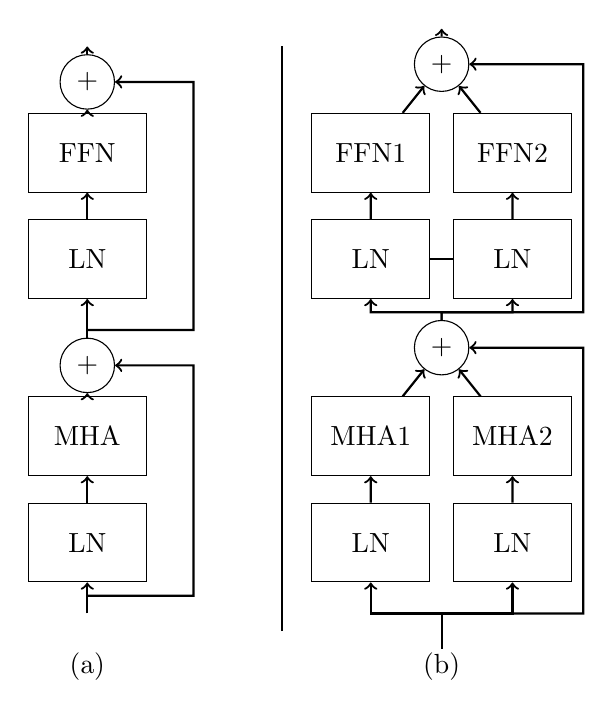
\begin{tikzpicture}[
    scale=0.90,
    block/.style={rectangle, draw, minimum width=1.5cm, minimum height=1cm},
    plus/.style={circle, draw, minimum size=0.6cm},
    arrow/.style={->, thick},
    skip/.style={->, thick}
]
% Left side (original)
% Addition node at the top (after MLP)
\node[plus] (plus2) at (0,6.5) {+};
% MLP block before final addition
\node[block] (mlp) at (0,5.5) {FFN};
% Post-attention layer norm
\node[block] (ln2) at (0,4) {LN};
% Multi-head attention block
\node[block] (mha) at (0,1.5) {MHA};
% Pre-attention layer norm
\node[block] (ln1) at (0,0) {LN};
% Addition node after first norm
\node[plus] (plus1) at (0,2.5) {+};
% Vertical connections
\draw[arrow] (0,-1) -- (ln1);  % Input arrow
\draw[arrow] (ln1) -- (mha);
\draw[arrow] (mha) -- (plus1);
\draw[arrow] (plus1) -- (ln2);
\draw[arrow] (ln2) -- (mlp);
\draw[arrow] (mlp) -- (plus2);
% Skip connections with right angles
\draw[skip] (0,-.75) -| (1.5,2.5) -- (plus1);
\draw[skip] (0, 3) -| (1.5,6.5) -- (plus2);
\draw[skip] (plus2) -- (0, 7);
% First vertical separation line
\draw[thick] (2.75,-1.25) -- (2.75,7);
% Right side (variant with parallel processing) - moved left by adjusting x-coordinates
% Final addition node
\node[plus] (plus2_var) at (5,6.75) {+};
% Parallel MLPs with increased vertical spacing
\node[block] (mlp1) at (4,5.5) {FFN1};
\node[block] (ln_mlp1) at (4,4) {LN};
\node[block] (mlp2) at (6,5.5) {FFN2};
\node[block] (ln_mlp2) at (6,4) {LN};
% Parallel MHAs with increased vertical spacing
\node[block] (mha1) at (4,1.5) {MHA1};
\node[block] (ln_mha1) at (4,0) {LN};
\node[block] (mha2) at (6,1.5) {MHA2};
\node[block] (ln_mha2) at (6,0) {LN};
% Addition node after parallel MHAs
\node[plus] (plus_mha) at (5,2.75) {+};
% Direct input connections to both LN1s
\draw[arrow] (5,-1) -| (ln_mha1);
\draw[arrow] (5,-1) -| (ln_mha2);
% MHA paths with right angles
\draw[arrow] (ln_mha1) -- (mha1);
\draw[arrow] (ln_mha2) -- (mha2);
\draw[arrow] (mha1) --  (plus_mha);
\draw[arrow] (mha2) --  (plus_mha);
% MLP paths with right angles
\draw[arrow] (ln_mlp1) -- (mlp1);
\draw[arrow] (ln_mlp2) -- (mlp2);
\draw[arrow] (mlp1) -- (plus2_var);
\draw[arrow] (mlp2) -- (plus2_var);
% Vertical connections between sections
\draw[arrow] (plus_mha) -- (5,3.25) -| (ln_mlp1);
\draw[arrow] (plus_mha) -- (5,3.25) -| (ln_mlp2);
\draw[arrow] (plus2_var) -- (5,7.25);
% Skip connections for right side
\draw[skip] (5,-1) -| (7,2.75) -- (plus_mha);
\draw[skip] (5,3.25) -| (7,6.75) -- (plus2_var);
\draw[thick] (5,-1.5) -- (5,-1);
\draw[thick] (ln_mlp1) -- (ln_mlp2);

\node (a) at (0, -1.75) {(a)};
\node (b) at (5, -1.75) {(b)};
\end{tikzpicture}
\caption{\label{fig:normal_and_pl_transformer_layer} \textbf{Comparing a normal transformer block with our layer parallel implementation.} In \textbf{(a)} we show a normal Transformer Layer. In \textbf{(b)} we illustrate our layer parallelization, where each column runs separately on one or multiple GPUs. The residuals are gathered and synchronized through a reduce operation across all GPUs. The pre-attention LayerNorms' weights are copied from the original blocks, while the post-attention LayerNorm's weights are averaged and shared in both layers.}
\end{figure}

\section{Related work}

\textbf{The effective depth of Deep Networks.} Theoretically, any feed-forward network with at least one hidden layer can model any function, given enough width \citep{Pinkus_1999}. In practice, it is easier to achieve high expressivity by increasing the model's depth. But naively increasing the depth can make things more difficult for the optimizer, since the gradients now have to flow through many layers. To alleviate this problem, ResNets \citep{he2015deepresiduallearningimage} introduced skip connections at regular intervals to allow an easy flow of the gradient to the first layers. Alternatively, in Inception \citep{szegedy2014goingdeeperconvolutions}, the researchers investigated ways to boost computational power by adding additional processing units along different parallel pathways in the computational network, rather than just along a single sequential path. A unification of both methods can be found in the Highway Networks \citep{srivastava2015highwaynetworks}, where the skip connection of the residual blocks consists of another block of compute. Nowadays, residual connections are ubiquitous in large models.


\begin{figure*}[h!]
  \centering
  \begin{subfigure}[b]{0.212\linewidth}
  \includegraphics[width=\textwidth,clip]{./figs/matrix_shuffle.pdf}
  \caption{Shuffling.}
  \label{fig:matrix-shuffling}
  \end{subfigure}
  \begin{subfigure}[b]{0.18\linewidth}
  \includegraphics[width=\textwidth,trim={1.3cm 0cm 0cm 0cm},clip]{./figs/matrix_identity.pdf}
  \caption{Pruning.}
  \label{fig:matrix-pruning}
  \end{subfigure}
  \begin{subfigure}[b]{0.18\linewidth}
  \includegraphics[width=\textwidth,trim={1.3cm 0cm 0cm 0cm},clip]{./figs/matrix_merge.pdf}
  \caption{Merging.}
  \label{fig:matrix-merge}
  \end{subfigure}
  \begin{subfigure}[b]{0.18\linewidth}
  \includegraphics[width=\textwidth,trim={1.3cm 0cm 0cm 0cm},clip]{./figs/matrix_parallel.pdf}
  \caption{Parallel.}
  \label{fig:matrix-parallel}
  \end{subfigure}
  \begin{subfigure}[b]{0.215\linewidth}
  \includegraphics[width=\textwidth,trim={1.3cm 0cm 0cm 0cm},clip]{./figs/matrix_parallel2_w_colorbar.pdf}
  \caption{2-Parallel.}
  \label{fig:matrix-2parallel}
  \end{subfigure}
\caption{\textbf{Changes in perplexity when applying transformations on contiguous stretches of layers.} Each one of the five heatmaps above correspond to a transformation of a group of consecutive layer, where the row index $s$ corresponds to the first layer of the group, and the column index $e$ to the last. The color coding indicates how the perplexity---estimated on a subset of RedPajama \citep{together2023redpajama}---is impacted by the corresponding modification of the model. The perplexity for the base Llama 2 7B model is $6.2$. In \textbf{(a)}, we shuffle---for each forward---the layers from $s$ to $e$. We can see that many consecutive layers can be shuffled with little impact on the overall perplexity. For instance, shuffling layers $15$ to $25$---$10$ layers in total---raises the perplexity only to $9.1$. In \textbf{(b)}, we prune contiguous stretches of layers. We can see that not many blocks can be removed without starting to significantly degrade the perplexity. In \textbf{(c)} we merge contiguous layers. The results with merging are near identical to those for pruning. This reveals there is no advantage in merging layers, most likely a results of averaging matrices not originating from the same initial values. In \textbf{(d)} we run contiguous blocks in parallel. Given the success of shuffling, it makes sense that this approach works well. Running blocks $17$ to $27$ raises the perplexity to $9.3$. Finally, in \textbf{(e)} we run \emph{pairs of consecutive layers} in parallel. As a result, we can parallelize much longer stretches of layers. For instance, we can apply this transformation from layer $4$ to $29$ and only increase the perplexity to $9.1$. This reduces the depth of the model from $32$ to $19$. This result makes it possible for us to leverage this parallelism for faster inference as we discuss in \S~\ref{sec:efficiency}.      
}
\label{fig:matrices}
\end{figure*}

% \textbf{The effective depth of DNNs.} Work on ResNet, work on LLMs.

\textbf{Efficient inference of LLMs.} Several complementary approaches exist for enhancing the computational efficiency of large-scale models, primarily through pruning and sparsity, quantization, and parallelism. Pruning\cite{LeCun1989OptimalBD, han2015learningweightsconnectionsefficient, han2016deepcompressioncompressingdeep, frantar2023sparsegpt} constitutes a dimensional reduction methodology that systematically eliminates redundant parameters while preserving model performance, thereby introducing architectural sparsity. This methodology is founded on empirical evidence demonstrating that neural networks frequently exhibit overparameterization, containing numerous weights with negligible contribution to the output. Through sophisticated pruning strategies, the inherent sparsity support in contemporary accelerators can be leveraged to enhance both memory utilization and computational efficiency \citep{zhang2020sparch, Spatten21}. In contrast, quantization encompasses the transformation of floating-point numerical representations (predominantly FP32) into reduced-precision integer formats, such as INT8 or INT4 \cite{han2016deepcompressioncompressingdeep, jacob2018quantization}. When implemented on hardware accelerators, these lower-precision representations facilitate superior memory bandwidth utilization, addressing a primary bottleneck in modern large-scale models \cite{gholami2024ai}; moreover, integer-based computations yield enhanced processing speed and substantially improved energy efficiency \cite{horowitz20141}. Finally, parallelization techniques during inference, such as tensor and pipeline parallelism, enable the distribution of computational workload across multiple devices, thereby reducing latency and increasing throughput, although this often requires careful consideration of communication overhead and load balancing \cite{li2024tpillmserving70bscalellms, narayanan2021efficientlargescalelanguagemodel}.





\textbf{Parallelism via Computational Graph Optimization.} Recent research has investigated architectural layer-level optimization strategies to enhance transformer model inference efficiency. The Staircase Transformer \citep{cutler2025stagformertimestaggeringtransformer} implements parallel layer execution with dynamic recurrent computation based on model requirements. Similarly, the Staggering Transformer \citep{cai2024medusasimplellminference} achieves layer parallelization by connecting layer $l_k$ at time step $t$ to both the $(t-1)$ output of layer $l_{k-1}$ and the $t$ output of layer $l_{k-2}$. To the best of our knowledge, no research has addressed the fusion of consecutive layers through tensor parallelism.


\section{Effective Depth}
\label{sec:effective-depth}

% Matrices plot
\begin{figure}[t]
    % \centering
    \begin{minipage}{0.9\textwidth}
    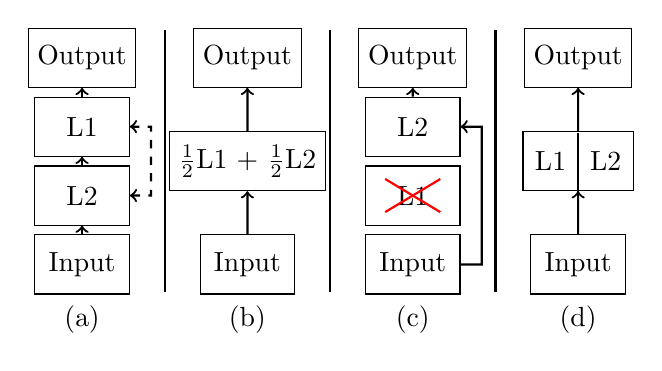
\begin{tikzpicture}[scale=0.7,
        box/.style={draw, rectangle, minimum width=1.2cm, minimum height=0.75cm},
        merged/.style={draw, rectangle, minimum width=1.4cm, minimum height=0.75cm},
        arrow/.style={->, thick},
        darrow/.style={<->, thick, dashed},
    ]
    
    % Left column (unchanged at x=0)
    \node[box] (input_left) at (0,0) {Input};
    \node[box] (layer1_left) at (0,1.25) {L2};
    \node[box] (layer2_left) at (0,2.5) {L1};
    \node[box] (output_left) at (0,3.75) {Output};
    
    \draw[arrow] (input_left) -- (layer1_left);
    \draw[arrow] (layer1_left) -- (layer2_left);
    \draw[arrow] (layer2_left) -- (output_left);
    \draw[darrow] (layer1_left) -| +(1.25,1.25) -- (layer2_left);
    \node (label_a) at (0, -1) {(a)};
    
    % First vertical separation line
    \draw[thick] (1.5,-0.5) -- (1.5,4.25);
    
    % Second column
    \node[box] (input_middle) at (3,0) {Input};
    \node[merged] (layers_middle) at (3,1.875) {$\frac{1}{2}$L1 + $\frac{1}{2}$L2};
    \node[box] (output_middle) at (3,3.75) {Output};
    
    \draw[arrow] (input_middle) -- (layers_middle);
    \draw[arrow] (layers_middle) -- (output_middle);
    \node (label_d) at (3, -1) {(b)};
    
    % Second vertical separation line
    \draw[thick] (4.5,-0.5) -- (4.5,4.25);
    
    % Third column
    \node[box] (input_right) at (6,0) {Input};
    \node[box] (layer1_right) at (6,1.25) {L1};
    \draw[red, thick] (5.5,0.95) -- (6.5,1.55);
    \draw[red, thick] (5.5,1.55) -- (6.5,0.95);
    \node[box] (layer2_right) at (6,2.5) {L2};
    \node[box] (output_right) at (6,3.75) {Output};
    
    \draw[arrow] (layer2_right) -- (output_right);
    \draw[arrow] (input_right) -- (7.25,0) -- (7.25,2.5) -- (layer2_right);
    \node (label_c) at (6, -1) {(c)};
    
    % Third vertical separation line
    \draw[thick] (7.5,-0.5) -- (7.5,4.25);
    
    % Fourth column
    \node[box] (input_far_right) at (9,0) {Input};
    \node[merged] (layers_far_right) at (9,1.875) {};
    \draw[thick] (9,0.75) -- (9,2.38);
    \node at (8.5,1.875) {L1};
    \node at (9.5,1.875) {L2};
    \node[box] (output_far_right) at (9,3.75) {Output};
    
    \draw[arrow] (input_far_right) -- (layers_far_right);
    \draw[arrow] (layers_far_right) -- (output_far_right);
    \node (label_b) at (9, -1) {(d)};
    
    \end{tikzpicture}
    \end{minipage}%
    % \begin{minipage}{0.5\textwidth}
    % \includegraphics[width=\textwidth]{figs/matrices.pdf}
    % \end{minipage}
    \hfill
    \begin{minipage}{0.45\textwidth}
    \label{fig:transform-diagrams}
    \caption{\textbf{Diagram of transformations applied in \S~\ref{sec:effective-depth}.} Diagrams \textbf{(a,b,c,d)} represent respectively shuffling, merging, pruning and parallel. %(b) The layer pair is merged into a single block by interpolating its weights (LERP). (c) The first layer is deactivated, reducing the depth of the LLM. (d) Two consecutive layers now share the same depth through Layer Parallelism.
    }
    \end{minipage}
\end{figure}

In this section, we investigate the effective depth of LLMs. By applying several transformations to a pretrained Transformer LLM, and measuring the resulting perplexity degradation, we reveal the loose dependencies between intermediary layers. The transformations consist of shuffling, merging, and pruning transformer layers. To avoid the combinatorial explosion resulting from considering all the possible subsets of transformer layers, we instead apply our transformations to all the contiguous stretch of layers. If $L=\{\ell_1, \ldots,\ell_N\}$ are the ordered layers, then we apply our transformations to all the sub-list $\{\ell_i\}_{i=s}^e$ with $1\leq s \leq e\leq N$. Previous works have shown that---at least when considering pruning---the importance of layers is well behaved, with low importance layers close to one another \citep{men2024shortgptlayerslargelanguage}, which justifies considering contiguous stretch of layers only. 

\textbf{Shuffling blocks.} We start by shuffling contiguous stretches of layers, re-ordering the layers according to random permutations. Results are shown in Fig.~\ref{fig:matrices}.(a). While shuffling the early and two last layers significantly raises the perplexity, there are large stretches of blocks which can be shuffled with surprisingly low impact on the perplexity. For instance, one can shuffle the layers $\{\ell_i\}_{15\leq i < 25}$ and only have a increase in perplexity of $2.9$. This goes against the classical belief that models build deeply hierarchical representations, where features in previous layers are leveraged to build more complex features in later layers. We interpret this as multiple layers working at the same level of abstraction. Using these insights, we define the \textit{effective depth} of an LLM as the shortest depth required to efficiently leverage existing latent representations without a significant loss of performance. This reveals an important level of  layer decoupling within the model.
%A similar observation has been made by \citep{lad2024remarkablerobustnessllmsstages} \matteo{check claim of paper}. % I couldn,t find this observation


\textbf{Running blocks in parallel.} The observed layer decoupling suggests that specific
transformer operations may be executed independently, providing an opportunity for parallel computation. More precisely,
let's consider two sequential transformer layers $\ell_{k}$ and $\ell_{k+1}$, each comprising attention and FFN sub-blocks ($A_k(\cdot)$ and $F_k(\cdot)$, respectively). The standard sequential output $\vy$ for these layers, given an input $\vx$, is given by:
\begin{align}
    \vy = \vx &+ \text{A}_k(\vx) \notag \\ 
              &+ \text{F}_k(\vx+ \text{A}_1(\vx)) \notag \\
              &+ \text{A}_{k+1}(\vx + \mathcolor{red}{\text{A}_k(\vx)} + \mathcolor{red}{\text{F}_k(\vx+ \text{A}_k(\vx))}) \notag \\
              &+ \text{F}_{k+1}(\vx + \mathcolor{red}{\text{A}_k(\vx)} + \mathcolor{red}{\text{F}_k(\vx+ \text{A}_k(\vx))} \\
              &+\text{A}_{k+1}(\vx + \mathcolor{red}{\text{A}_k(\vx)} + \mathcolor{red}{\text{F}_k(\vx+ \text{A}_k(\vx))})) \tag{SEQ}\label{eq:seq}
\end{align}
The highlighted terms represent the first block's contribution to the second block's processing. Given the observed layer independence, we can hypothesize that these terms have minimal impact, leading to the following approximation:
\begin{align}
    \hat{\vy} = \vx &+ \text{A}_k(\vx) + \text{F}_k(\vx+ \text{A}_k(\vx)) \\
    &+ \text{A}_{k+1}(\vx) + \text{F}_{k+1}(\vx + \text{A}_{k+1}(\vx)) \tag{PAR}\label{eq:par}
\end{align}
This approximation enables parallel execution of blocks $\ell_{k}$ and $\ell_{k+1}$ through divergent computational paths. 
%Compared to pruning, running blocks in parallel reduces the effective depth without reducing the parameter count. 
We experiment with running contiguous stretches of layers in parallel and show our results in Fig.~\ref{fig:matrix-parallel}. We observe results similar to shuffling. Unlike shuffling, this approach allows us to potentially improve the runtime through enhanced parallelism. We show how we can, for instance, run layers $17$ to $27$ in parallel, only losing $3.1$ perplexity points, while reducing the depth of the model from $32$ to $23$. 

\textbf{Contiguous 2-parallel.} Instead of parallelizing long stretches of layers, we experiment with running \emph{pairs of consecutive layers} in parallel. This springs from the assumption that local ordering matters less than global ordering, i.e. shuffling consecutive layers is less risky than shuffling layers further apart. As an example, if we apply the proposed transformation to layers $\{\ell_{15},\ell_{16},\ell_{17},\ell_{18},\ell_{19}\}$, it would result in the following process: (1) the two layers $\{\ell_{15},\ell_{16}\}$ process the input in parallel (according to equation \eqref{eq:par}), (2) the output is forwarded to layers $\{\ell_{17},\ell_{18}\}$ which process it in parallel; finally, in (3) their joint output is fed to layer $\ell_{19}$ which processes it on its own as any normal layer. The effect of such transformation of the compute graph on the perplexity can be seen in Fig.~\ref{fig:matrix-2parallel}. Remarkably, it is possible to run wide stretches of consecutive pairs of blocks in parallel with only a minor degradation of perplexity. For instance, one can apply this transformation from layer $4$ to layer $29$ with only a degradation of perplexity of $2.9$, while reducing the model depth from $32$ to $19$. The success of this approach led us to also try running triplets of consecutive layers in parallel, but we found it to perform less well.    


\textbf{Exploring other transformations.} We also experiment with pruning (Fig.~\ref{fig:matrix-pruning}) and merging (Fig.~\ref{fig:matrix-merge}). Pruning has already been studied in several prior works \citep{gromov2024unreasonableineffectivenessdeeperlayers, jung2019compactassessingcompactnessrepresentations}. While pruning a layer leads to a larger perplexity increase compared to parallelizing two blocks, it offers the advantage of reducing the model's parameter count, which results in improved throughput and more efficient memory usage.

% \matteo{TODO: We compare the gains obtained with our approach to those obtained through pruning in \S~\ref{todo}.} Merging gives near identical results to pruning. This reveals that merging different layers together deteriorates them significantly. 

\section{Efficient Parallelization of Blocks}
\label{sec:efficiency}

% LP and TP tikz
\begin{figure*}[t]
\centering
\usetikzlibrary{backgrounds}

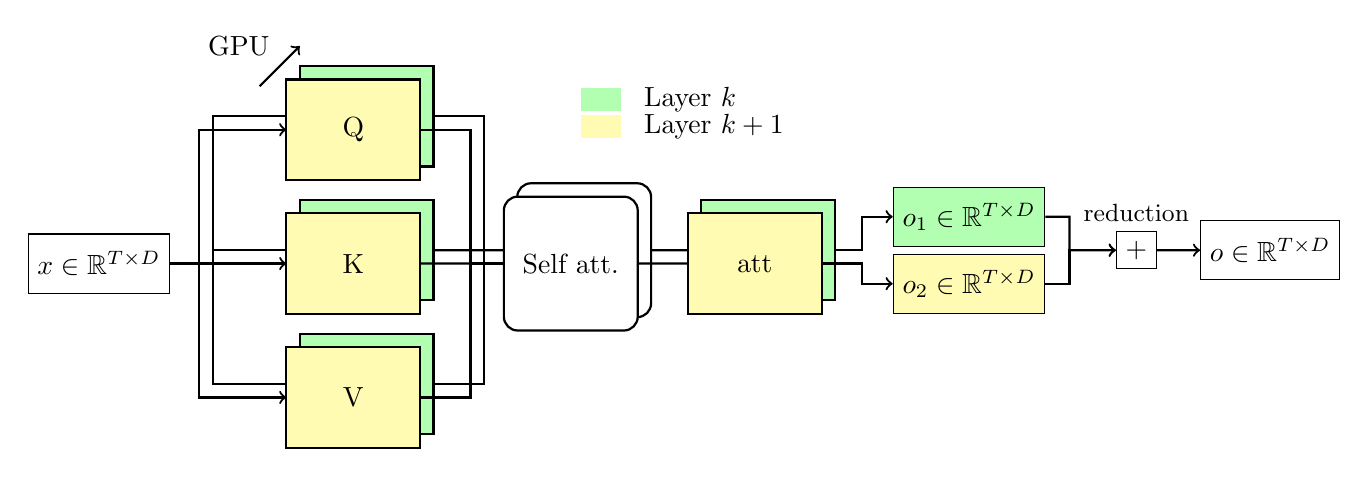
\begin{tikzpicture}[scale=0.85,
        box/.style={draw, rectangle, minimum width=1.5cm, minimum height=0.75cm},
        reducebox/.style={draw, rectangle, minimum width=0.3cm, minimum height=0.3cm},
        arrow/.style={->, thick},
        line/.style={-, thick},
    ]
    % Add diagonal GPU arrow
    \draw[->, thick] (2.4, 3.2) -- node[above left] {GPU} (3, 3.8);
    
    % Add color legend
    \node[rectangle, fill=green!30, minimum width=0.5cm, minimum height=0.3cm] at (7.5, 3) {};
    \node[right] at (8, 3) {Layer $k$};
    \node[rectangle, fill=yellow!30, minimum width=0.5cm, minimum height=0.3cm] at (7.5, 2.6) {};
    \node[right] at (8, 2.6) {Layer $k+1$};
    
    \node[box] (input) at (0, 0.55) {$x\in\mathbb{R}^{T\times D}$};

    \stackedtworectangles[3,-2]{V}{green!30}{yellow!30}{V};
    \stackedtworectangles[3,0]{K}{green!30}{yellow!30}{K};
    \stackedtworectangles[3,2]{Q}{green!30}{yellow!30}{Q};
    \draw[arrow] (input) -- +(1.5,0) |- (Q-E2left);
    \draw[arrow] (input) -- +(1.5,0) |- (K-E2left);
    \draw[arrow] (input) -- +(1.5,0) |- (V-E2left);

    % Move E1 arrows to the background
    \begin{scope}[on background layer]
        \draw[arrow] (input) -- +(1.7,0) |- (Q-E1left);
        \draw[arrow] (input) -- +(1.7,0) |- (K-E1left);
        \draw[arrow] (input) -- +(1.7,0) |- (V-E1left);
    \end{scope}

    % Hack
    \draw[line] (5.6, 0.55) -- (6.5, 0.55);    
    \draw[line] (5.6, 0.75) -- (6.5, 0.75);

    \stackedroundedtworectangles[6.25, -0.25]{mha}{white}{white}{Self att.};

    % Draw the rectangle or other elements AFTER the arrow
    \stackedtworectangles[9, 0]{att}{green!30}{yellow!30}{att};
    \draw[line] (Q-E2right) -- +(0.75, 0) |- (mha-E2left);
    \draw[line] (K-E2right) --  (mha-E2left);
    \draw[line] (V-E2right) -- +(0.75, 0) |- (mha-E2left);

    % Move E1 arrows to the background
    \begin{scope}[on background layer]
        \draw[line] (Q-E1right) -- +(0.75, 0) |- (mha-E1left);
        \draw[line] (K-E1right) --  (mha-E1left);
        \draw[line] (V-E1right) -- +(0.75, 0) |- (mha-E1left);
    \end{scope}

    \draw[line] (mha-E2right) -- (att-E2left);
    \node[box, fill=green!30] (o1) at (13, 1.25) {$o_1\in\mathbb{R}^{T\times D}$};
    \node[box, fill=yellow!30] (o2) at (13, 0.25) {$o_2\in\mathbb{R}^{T\times D}$};
    \draw[arrow] (att-E2right) -- +(.6, 0) |- (o2);

    % Move E1 arrows to the background
    \begin{scope}[on background layer]
        \draw[arrow] (att-E1right) -- +(0.4, 0) |- (o1);
        \draw[arrow] (mha-E1right) -- (att-E1left);
    \end{scope}
    
    % Add allreduce box
    \node[reducebox] (allreduce) at (15.5, 0.75) {$+$};
    \node[above] at (allreduce.north) {\small reduction};
    
    % Add arrows from o boxes to allreduce
    \draw[arrow] (o1) -- +(1.5,0.0) |- (allreduce);
    \draw[arrow] (o2) -- +(1.5,0.0) |- (allreduce);
    
    % Add final output box
    \node[box] (output) at (17.5, 0.75) {$o\in\mathbb{R}^{T\times D}$};
    \draw[arrow] (allreduce) -- (output);
\end{tikzpicture}
\caption{\label{fig:lp2} \textbf{Layer Parallel (LP) implementation of attention}. In this diagram, the stacked layers represent different GPUs, the colors indicate the intermediate tensors of different layers and the arrows express linear projections. In this case, the number of GPUs and the number of parallelized layers coincides and is 2, which is the set-up that we use for all our experiments in this work. We see how tensors for the two layers are distributed across the two GPUs. We also notice the reduction step happening at the end, summing the outputs from each GPUs, which differs from the regular computational graph obtained when running layers in parallel as in equation \eqref{eq:par}. }
\end{figure*}


\textbf{Naive block parallelization.} Pure parallelization of  two transformer blocks would consist in implementing equation \eqref{eq:par}. To optimize our parallel implementation, we need to leverage efficient GPU kernels by e.g. concatenating together matrices from different blocks. As an example, let's consider parallelizing $\vy_1 = W_1 \vx$ and $\vy_2 = W_2 \vx$, $\vx\in \mathbb{R}^{d_x}, \vy\in \mathbb{R}^{d_y}, W_1,W_2\in \mathbb{R}^{d_y\times d_x}$. We can concatenate $W=[W_1,W_2]\in \mathbb{R}^{2*d_y\times d_x}$ and get $[\vy_1,\vy_2]=W \vx$. However, this would not work if, instead of a shared input $\vx$, we had two separate inputs $\vx_1$ and $\vx_2$. This is precisely the situation we are in when we apply different layer norms to the input of the two attention blocks. The Feed-Forward Networks (FFN) also have different inputs, in addition to having different layer norms. Those considerations directed us to modify the computational graph of the parallel processing of blocks. While we differ from equation \eqref{eq:par}, we show that our approach nonetheless---and quite surprisingly---works well on already trained models, circumventing the need to train from scratch.


\textbf{The hardware limits of parallelisms.} Another difficulty we faced when parallelizing transformer blocks is the saturation of GPU resources. LLM inference typically saturates GPU resources due to its intensive compute and memory bandwidth requirements. When all the GPU cores are already being utilized by one matrix multiplication, running another matrix multiplication in parallel can be as slow as running them sequentially. This is the case with large transformer models, as even processing a single sequence can fully utilize a GPU's capabilities. As such, simply attempting to run two blocks in parallel would result in sequential execution, as the scheduler would allocate operations from both blocks to the same job stream.
To achieve true parallel execution of layers, we decided to leverage Tensor Parallelism by distributing layer weights across multiple GPUs.

We extend the tensor parallelism scheme introduced in Megatron \cite{shoeybi2020megatronlmtrainingmultibillionparameter} to incorporate our novel Layer Parallelism. Below, we detail our approach for each major component of the transformer block, initially setting aside Layer Normalization considerations and tackling the Multi-Head Attentions (MHA) and the FFN. Our approach is also illustrated in Fig.~\ref{fig:normal_and_pl_transformer_layer}. It is important to note that the resulting computational graph is not numerically equivalent to the original architecture. This numerical discrepancy stems from the positioning of the pre-normalization operations that precede each transformer sub-block.

% \matteo{I think we should still emphasize better how our method is not entirely equivalent to running blocks in parallel. Indeed, we altered the computational graph for better efficiency.}


\textbf{Layer Parallel Multi-Head Attention.} Traditional tensor parallelism in MHA distributes attention heads evenly across GPUs, performing self-attention and output projection locally before gathering results through worker summation. Each GPU processes tensors of dimensions $Q,K,V,att\in\mathbb{R}^{T\times \frac{D}{g}}$, where $T$ is sequence length, $D$ is feature dimension, and $g$ is the number of parallel workers. The local output projection produces $o_i\in\mathbb{R}^{T\times D}$ for each worker $i$, with rank $\frac{D}{g}$ until the gather operation restores full rank. To implement Layer Parallelism, we increase the depth of the query, key, and value weight matrices ($W_Q,W_K,W_V\in\mathbb{R}^{(g_n\cdot h_d)\times D}$) and widen the output projection ($W_O\in\mathbb{R}^{D\times (n_h\cdot h_d)}$), where $n_h$ represents heads per GPU and $h_d$ is head dimensionality. The reduction operation now will simultaneously compute the full-rank output projections and the sum of all parallel layers (Fig.~\ref{fig:lp2}(b)). 

%\matteo{Here it is a bit confusing because we do not mention the reduction at the end. Also we should link to Fig.5}

\textbf{Layer Parallel Feed Forward Network.} Standard tensor parallelism for single-hidden-layer FFNs splits the first layer's output across devices, generates partial outputs from the second layer, and combines them through reduction. To parallelize two FFN layers, we double the first layer's output dimensionality and perform separate output projections for each layer. A single reduction operation then serves the dual purpose of computing full outputs for each layer and combining their results, as shown in Fig.~ \ref{fig:normal_and_pl_transformer_layer}(b). In summary, Layer Parallelism for FFN just concatenates the up-projection weights and continues as normal TP, allowing for multiple GPUs to be allocated per parallelized layer.

% \matteo{so effectively we can describe this by saying we concat the tensor and then proceed like a normal tensor parallelism, right?}

\textbf{Handling Layer Normalization.} Layer Normalization presents unique challenges since these layers were trained on specific input distributions. For MHA pre-normalization, we apply separate normalization on each device. For FFN pre-normalization, we found that linearly interpolating the weights of both FFN pre-norms yielded better perplexity than maintaining separate normalizations. This improvement may stem from the fact that, given we reduce the MHA outputs over the parallelized layers, interpolation effectively combines the expected input distributions of both layers.

%In most circumstances, running LLM inference on a hardware accelerator such as a GPU makes full utilization of its resources due to the high quantity of dense compute and memory bandwidth required. Even the forward pass of a single sequence can saturate the accelerator. If we naively tried to run two blocks in parallel, the scheduler will just allocate the operations of both blocks in the stream of jobs and they would end up being executed sequentially.

%To exploit the parallelization of entire layers, we have to resort to Tensor Parallelism, splitting the weights of each layer in the transformer, and thus dividing the work done by each GPU on each block. We extend the tensor parallelism scheme for Transformer models introduced in Megatron \cite{shoeybi2020megatronlmtrainingmultibillionparameter} to account for Layer Parallelism. Let's consider a Transformer block (Figure \ref{fig:normal_and_pl_transformer_layer}(a)) and for now forget about the Layer Normalizations:

%\textbf{Layer Parallel Multi-Head Attention (MHA)}. The common way of achieving tensor parallelism within the MHA block is to distribute to each GPU the same number of heads, perform the self-attention and output projection locally, and then gather the output result by summing the partial outputs from all workers. In this setting, $Q,K,V,att\in\mathbb{R}^{T\times \frac{D}{g}}$ where $T$ is the sequence length, $D$ is the feature dimension and $g$ is the number of parallel workers. The local output projection computes the result $o_i\in\mathbb{R}^{T\times D}$ for each worker $i$. Note that this matrix has rank $\frac{D}{g}$, and the full-rank will be recovered after the gather operation. To introduce Layer Parallelism in this formulation, we can just increase the depth of $W_Q,W_K,W_V$ and the width of the output projection $W_O$ such that $W_Q,W_K,W_V\in\mathbb{R}^{(g_n\cdot h_d)\times D}$ and $W_O\in\mathbb{R}^{D\times (n_h\cdot h_d)}$, where $n_h$ is the number of heads per GPU, and $h_d$ is the head dimensionality.

%\textbf{Layer Parallel Feed Forward Network (FFN).} Tensor Parallelism on Feed Forward Networks with one hidden layer are efficiently implemented by splitting the output of the first layer across multiple devices, and generating full low-rank outputs from the second layer and summing them with a reduce operation. To compute two separate FFN layers at the same time, we can increment the dimensionality of the output of the first layer by the number of parallelized layers (2 in our case), and then perform two different output projections on those. Then sum all the outputs with the reduce operation. Note that for both the FFN and the MHA, the reduce operation serves to both compute the full output for each layer as well as summing the outputs of both layers, as depicted in Figure \ref{fig:normal_and_pl_transformer_layer}(b). 

%\textbf{Handling the Layer Normalizations.} Without taking into account the pre-normalization blocks, so far our parallel transformer block is numerically equivalent. But the Layer Normalizations pose a challenge, since they were trained to 'see' the distribution of their own inputs. Nevertheless, for the MHA pre-norms we apply its own normalization on each device. For the FFN pre-norm, we find that taking a linear interpolation of the weights of both FFN pre-norms yielded slightly better results in the measured perplexity than having them separate. This could be explained by the fact that since the layers are already decoupled, by talking the interpolation we are combining the distributions that the inputs at both layers would have.

% Recent studies have demonstrated that transformer layers in LLMs exhibit functional specialization at different depths. Our empirical analysis reveals that certain layers demonstrate robustness to positional shuffling (Figure \ref{fig:matrices}a). Upon this observation, we question whether some of the layers in the transformer do not provide useful for the computation of the output tokens. Figure \ref{fig:matrices}c shows that skipping a small number of layers quickly degrades performance, removing this notion.\\

% The observed layer decoupling suggests that specific transformer operations may be executed independently, providing an opportunity for parallel computation. We first test the naive solution of merging consecutive groups of 2 layers using linear interpolation (Figure \ref{fig:matrices}b). But it can be seen that this naive method quickly makes the perplexity worse as we stack for merged layers. Instead of combining two independent layers onto a single one, we ask ourselves if by running two consecutive layers independently but with the same input (Figure \ref{fig:normal_and_pl_transformer_layer}b) we can elude this fast perplexity degradation. Surprisingly, as seen on Figure \ref{fig:matrices}d, we can stack multiple pairs of layers that compute their residuals independently while keeping the perplexity close to the unmodified LLM.\\

% We propose leveraging this property to optimize LLM inference through Layer Parallelism (LP), a technique that restructures the computational graph of an already trained LLM to enable concurrent execution of consecutive transformer layers.\\


\section{Experiments \& Results}


\begin{table*}[h]
\centering
\footnotesize
\begin{tabular}{cc|ccccccc}
\hline
Effective Depth & Par. Layers & MMLU & PiQA & Arc Easy & Arc Challenge & Winogrande & openbooqka & hellaswag \\
\hline
\multicolumn{9}{c}{\textbf{Llama 2 7B}}\\
\hline
32 (Baseline) & - & 0.4583 & 0.8009 & 0.8106 & 0.5196 & 0.7411 & 0.4520 & 0.7821 \\
% Llama-2-7B & 16-24 (Ours) & 0.4561 & 0.7884  & 0.8013 & 0.5077 & 0.7372 & 0.4400 & 0.7741\\
% Llama-2-7B & 15-25 (Ours) & 0.4509 & 0.7960 & 0.7845 & 0.5068 & 0.7395 & 0.4460 & 0.7731 \\
27  (Ours) & 18-28 & 0.4625 & 0.7933 & 0.8005 & 0.5094 & 0.7348 & 0.4600 & 0.7782 \\
26  (Ours) & 16-28 & 0.4588 & 0.7927 & 0.7976 & 0.4983 & 0.7340 & 0.4460 & 0.7745 \\
25  (Ours) & 14-28 & 0.4532 & 0.7851 & 0.7917 & 0.4949 & 0.7340 & 0.4440 & 0.7673 \\
24  (Ours) & 12-28 & 0.4083 & 0.7845 & 0.7841 & 0.4839 & 0.7190 & 0.4360 & 0.7578 \\
23  (Ours) & 10-28 & 0.3519 & 0.7829 & 0.7677 & 0.4488 & 0.6922 & 0.4240 & 0.7368 \\
\hline
\multicolumn{9}{c}{\textbf{Llama 3.2 3B}}\\
\hline
28 (Baseline) & - & 0.5610 & 0.7992 & 0.7807 & 0.4872 & 0.7214 & 0.4520 & 0.7557 \\
% Llama-3.2-3B & 16-24 (Ours) & 0.5469 & 0.7840 & 0.7601 & 0.4693 & 0.7222 & 0.4180 & 0.7370 \\
24 (Ours) & 17-25 & 0.5508 & 0.7856 & 0.7521 & 0.4753 & 0.7167 & 0.4420 & 0.7384 \\
23  (Ours) & 15-25 & 0.5481 & 0.7748 & 0.7399 & 0.4735 & 0.7119 & 0.4200 & 0.7303 \\
22  (Ours) & 13-25 & 0.4693 & 0.7666 & 0.7264 & 0.4497 & 0.6914 & 0.4180 & 0.7193\\
21  (Ours) & 11-25 & 0.3890 & 0.7519 & 0.6839 & 0.4061 & 0.6638 & 0.4020 & 0.6847 \\
20  (Ours) & 9-25 & 0.3107 & 0.7416 & 0.6481 & 0.3652 & 0.6227 & 0.3620 & 0.6407 \\
\hline
\end{tabular}
\caption{\label{tab:model-comparison}\textbf{5-shot In-Context Learning accuracies across standard benchmarks}. Effective Depth shows the minimum number of sequential operations from input to output. Par. Layers indicates the range of consecutive layers where pairs were processed in with Layer Parallelism.}
\end{table*}

\begin{table}[h]
\centering
\footnotesize
\begin{tabular}{c|cc}
Finetuning Steps & MMLU & Rel. MMLU (\%)\\
\hline
0 (Baseline) & 0.5610 & 100 \\
\hline
0 (13-25 LP) & 0.4693 & 83.6  \\
4096 (Ours) &  0.4979 & 88.8 \\
8192 (Ours) & 0.5295 & 94.4 \\
16384 (Ours) & 0.5222 & 93.1\\
32736 (Ours) & 0.5266 & 93.8
\end{tabular}
\caption{\label{tab:finetuning} \textbf{Recovery of MMLU accuracy through finetuning on Llama 3.2 3B with Layer Parallelism applied to layers 13-25.} Relative MMLU shows performance as a percentage of the baseline model's accuracy. The recovered MMLU saturates after fine-tuning for 8k steps.}
\end{table}

% delta should nb of layers grouped into pairs
% add conclusion to caption
\begin{figure*}[h!]
  \centering
  \begin{subfigure}[b]{0.4\linewidth}
  \includegraphics[width=\textwidth,clip]{./figs/llama2_7b_comparison_ppl.pdf}
  \caption{Llama2 7B.}
  \end{subfigure}
  \hspace{2em}
  \begin{subfigure}[b]{0.4\linewidth}
  \includegraphics[width=\textwidth,clip]{./figs/llama3_3b_comparison_ppl.pdf}
  \caption{Llama3.2 3B.}
  \end{subfigure}
\vspace{-0.2cm}
\caption{\textbf{Perplexity when running pairs of consecutive layers in parallel.} Perplexity of Llama2 7B and Llama3.2 3B models on the test set of RedPajama\cite{together2023redpajama} when applying Layer Parallelism to $\Delta$ consecutive layers. The parallelized interval for each data point is $[\text{end index} - \Delta, \text{end index}[$.      
}
\label{fig:llama_ppl_sweep}
\end{figure*}

% \begin{figure*}[t]
% \centering
% \includegraphics[width=0.95\textwidth]{figs/llama_comparison_ppl.pdf}
% \caption{\label{fig:llama_ppl_sweep} Perplexity of Llama 2 7B and Llama 3.2 3B models on the test set of RedPajama\cite{together2023redpajama} when applying Layer Parallelism to $\Delta$ consecutive layers. The parallelized interval for each data point is $(\text{end index} - \Delta, \text{end index})$.}
% \end{figure*}


\begin{figure*}[h]
\centering
\includegraphics[width=0.97\textwidth]{figs/average_time_ms.pdf}
\caption{\label{fig:tp_avg_time} \textbf{Wall clock time to complete the following inference tasks}: KV Cache pre-filling for a given sequence length, autoregressive generation up to the indicated sequence length, and single token generation with a pre-filled KV Cache of the indicated sequence length. The baseline is the original model with all layers making use of Tensor Parallelism. The Parallel Layers number ($\Delta$) indicates how many layers have been merged using Layer Parallelism (e.g. a $\Delta$ of 4 indicates that 2 groups of 2 layers have been converted to 2 effective layers). The gains in inference speed are directly proportional to the grade of Layer Parallelism. The 1-token generation task for Llama 3.2 3B does not saturate the GPU compute until a sequence length of 2048. Even in this regime, Layer Parallelism benefits from considerable speed-ups.}
\end{figure*}

In this section, we evaluate Layer Parallelism across three dimensions: inference speed improvements, impact on In-Context Learning performance, and the potential to recover model accuracy through targeted fine-tuning of parallelized layers.

\textbf{Experimental protocol.} For all our experiments, we use a node with two A100 SXM4 80Gb GPUs, four AMD EPYC 7742 CPUs, and 512Gb of RAM. We test for varying sequence lengths, up to $4096$ (Llama's context window), with a batch size of $1$ unless indicated otherwise. We consider two models of the Llama family: Llama2 7B, and Llama3.2 3B.  We always apply Layer Parallelism of $2$ (one layer to each GPU) on the merged sequential layers and apply Tensor Parallelism as described in \citep{shoeybi2020megatronlmtrainingmultibillionparameter} for the rest. The baselines are fully Tensor Parallel Llama models. For evaluation, we measure the ICL 5-shot accuracies using the \verb|lm-eval| package \citep{eval-harness}. We test the ICL accuracy of the models on several tasks: MMLU \citep{hendrycks2021measuringmassivemultitasklanguage}, PiQA \citep{bisk2019piqareasoningphysicalcommonsense}, ARC Easy, ARC Challenge, Winogrande \citep{sakaguchi2021winogrande}, OpenBookQA \citep{mihaylov2018suitarmorconductelectricity} and Hellaswag \citep{zellers2019hellaswag}. The perplexity (PPL) of the models is always evaluated against a subset of the test set of RedPajama \citep{together2023redpajama}.

\textbf{Impact of layer-parallelism on PPL and ICL accuracies.} We begin by exploring the evolution of the perplexity when applying layer parallelism to stretches of layers of varying lengths, and starting at different depths. Results in Fig.~\ref{fig:llama_ppl_sweep} show how both models---Llama2 7B and Llama3.2 3B---exhibit a common sequence ending index for which the perplexity is minimized, which is 28 and 25 for Llama2 7B and Llama3.2 3B, respectively. Taking this into consideration, in Table \ref{tab:model-comparison} we evaluate the In-Context Learning capabilities of models of different effective depths, for which parallelized sequences end at those indices. For Llama 2 7B we observe that applying Layer Parallelism to a sequence greater than 14 layers results in a steep loss of In-Context Learning capabilities in the more challenging benchmarks, like MMLU. Likewise, parallelizing above  10 layers of Llama 3.2 3B sees an even more rapid decrease in performance on difficult benchmarks. The effective depth of both models at the parallel configurations before those sudden drops in performance is 25 and 23, a reduction of 21\% and 18\% of their original depths, respectively.

% \textbf{Impact on the inference speed.} We run an ablation over several configurations and input sequence lengths on Figure \ref{fig:tp_avg_time} to test the speed on three different tasks: KV-Cache pre-filling, autoregressive generation up to the sequence length(with KV-Cache) and 1-token generation with a pre-filled KV-Cache of the corresponding sequence length. Our ablations show that the speed gain is directly proportional to the reduction of the effective depth of the model. For the effective depths of 25 ($\Delta=14$) in Llama 2 7B, we observe an average speed-up of 14\% at the largest sequence length in the 1-token generation task. Likewise, for an effective depth of 23 ($\Delta=10$) in Llama 3.2 3B, we report a speed-up of 10.5\%. For more aggressive parallelism, $\Delta=18$ and $\Delta=16$, we report a speed-up of 18.2\% and 15.7\%, at the expense of a large drop in ICL accuracy.

\textbf{Impact on the inference speed.} We run an ablation over several configurations and input sequence lengths on Figure \ref{fig:tp_avg_time} to test the speed on three different tasks: KV-Cache pre-filling, autoregressive generation up to the sequence length(with KV-Cache) and 1-token generation with a pre-filled KV-Cache of the corresponding sequence length. Our ablations show that the speed gain is directly proportional to the reduction of the effective depth of the model. For the effective depths of 25 ($\Delta=14$) in Llama 2 7B, we observe an average speed-up of 1.29x at the largest sequence length in the 1-token generation task. Likewise, for an effective depth of 23 ($\Delta=10$) in Llama 3.2 3B, we report a speed-up of 1.22x. For more aggressive parallelism, $\Delta=18$ and $\Delta=16$, we report a speed-up of 1.38x and 1.35x , at the expense of a large drop in ICL accuracy.

% \textbf{Impact on memory usage.} Similarly to compute times, the memory decreases linearly when the number of parallelized layers increases. This memory consumption reduction comes from 

\textbf{Fine-tuning for performance recovery.} While Layer Parallelism offers significant speed improvements, the architectural modifications can impact model performance. To address this, we investigated whether fine-tuning could recover the original model's capabilities. Using Llama 3.2 3B with Layer Parallelism applied to layers 13-25 ($\Delta=12$), we fine-tuned only the parallelized layers on random samples from RedPajama's training set \cite{together2023redpajama}. With a batch size of 2 and a learning rate of $1e-4$, we observed substantial recovery of model performance. As shown in Table \ref{tab:finetuning}, fine-tuning for 8,192 steps improved MMLU accuracy from 83.6\% to 94.4\% of the baseline performance, demonstrating that much of the model's original capability can be recovered while maintaining the speed benefits of Layer Parallelism.

\section{Limitations}

% Need multiple GPUs and tensor parallelism to work. Performance might be dependant on the workload and configuration of the cells.
% We only do the ablations on batch_size=1 due to memory limitations, and
% We don't test the interplay of quantization strategies with our method
% Does not work as well on small models, likely due to the less sparse 
% There's always some performance drop
% Performance drops after some depth
% Even though some performance can be retrieved through finetuning, it's not as high as the baseline model.
% There is no way of finding the 'true' effective depth.

While our approach demonstrates significant improvements in inference efficiency, several important limitations should be considered. 

%\textbf{The method requires multiple GPUs} with tensor parallelism capabilities which may not be available in all deployment scenarios. The performance benefits are also heavily dependent on specific workload characteristics and hardware configurations, potentially limiting the generalizability of our reported improvements.

%\textbf{Our experimental evaluation faced certain constraints.} Due to memory limitations, we conducted ablation studies only with batch size 1, which may not fully represent real-world deployment scenarios where larger batch sizes are common. Additionally, we did not investigate the interaction between our method and various quantization strategies, leaving open questions about potential complementary or competing effects.

\textbf{The effectiveness of our approach exhibits notable variations across model scales.} Smaller models show reduced benefits, likely due to their less sparse activation patterns and more tightly coupled layer dependencies. Even in successful cases, we observe a consistent, albeit small, performance degradation compared to the baseline. This degradation becomes more pronounced as model depth increases, suggesting a practical upper limit to the number of layer pairs that can be effectively parallelized.

\textbf{Finetuning.} While some performance loss can be mitigated through fine-tuning, we were unable to fully recover the baseline model's performance levels. This suggests fundamental trade-offs between computational efficiency and model capability that cannot be entirely eliminated through optimization. 

\textbf{Determining the 'true' effective depth—the optimal configuration of parallel layer pairs—remains an open challenge} as there is no theoretical framework for predicting the optimal grouping strategy.
These limitations highlight important directions for future research, particularly in developing more robust methods for determining optimal layer groupings and investigating the interplay between our approach and other efficiency-oriented techniques.

%This section aims to cut the grass under the reviewers' feet, i.e. we know the limitations of our method/experiments, but they do not remove all the merit of our project. 

\section{Conclusion}

In this work, we presented Layer Parallelism, a novel approach that exploits independence patterns between transformer layers to optimize LLM inference. By restructuring the computational graph to enable parallel execution of consecutive layer pairs through tensor parallelism, we achieved substantial speed improvements without model retraining. Our method reduced the effective depth of Llama 2 7B by 21\% while maintaining strong performance, yielding up to a 1.29x improvement in inference speed for single-token generation with long sequences. Similar benefits were observed with Llama 3.2 3B, achieving an 18\% reduction in effective depth with up to a 1.22x speed-up. Moreover, we show that we can recover 10.8\% of ICL accuracy on MMLU by fine-tuning the parallelized models using few resources.

These results challenge the conventional view that transformer layers must process information strictly sequentially, suggesting instead that certain layers can operate independently without significant performance loss. From a practical standpoint, LP offers a straightforward approach to improve inference efficiency in production environments. Future work could focus on developing theoretical frameworks to predict optimal layer groupings, investigating interactions with other efficiency techniques such as quantization, and understanding the fundamental principles behind layer independence. Despite its limitations, LP represents a practical advancement in making LLM deployment more efficient and economically viable.

% Future research: put in pipeline parallelism schedulers -> LP in different nodes of accelerated inference; Finetuning? Try on bigger and smaller models, and models trained on more data.

\section*{Impact Statement}

% Authors are \textbf{required} to include a statement of the potential 
% broader impact of their work, including its ethical aspects and future 
% societal consequences. This statement should be in an unnumbered 
% section at the end of the paper (co-located with Acknowledgements -- 
% the two may appear in either order, but both must be before References), 
% and does not count toward the paper page limit. In many cases, where 
% the ethical impacts and expected societal implications are those that 
% are well established when advancing the field of Machine Learning, 
% substantial discussion is not required, and a simple statement such 
% as the following will suffice:

% ``This paper presents work whose goal is to advance the field of 
% Machine Learning. There are many potential societal consequences 
% of our work, none which we feel must be specifically highlighted here.''

% The above statement can be used verbatim in such cases, but we 
% encourage authors to think about whether there is content which does 
% warrant further discussion, as this statement will be apparent if the 
% paper is later flagged for ethics review.

This paper presents work whose goal is to advance the field of 
Machine Learning. There are many potential societal consequences of our work, none of which we feel must be specifically highlighted here.

\bibliography{bibliography}
\bibliographystyle{icml2024}
\clearpage


%%%%%%%%%%%%%%%%%%%%%%%%%%%%%%%%%%%%%%%%%%%%%%%%%%%%%%%%%%%%

\onecolumn
\appendix


\section{Ablation: Memory efficiency}

\begin{figure*}[!h]
\centering
\includegraphics[width=\textwidth]{figs/peak_memory_mb.pdf}
\caption{\label{fig:tp_avg_time} Maxiumum memory usage (Mb) to complete the following inference tasks: KV Cache pre-filling for a given sequence length, autoregressive generation up to the indicated sequence length, and single token generation with a pre-filled KV Cache of the indicated sequence length. The baseline is the original model with all layers making use of Tensor Parallelism. The Parallel Layers number ($\Delta$) indicates how many layers have been merged using Layer Parallelism (e.g. a $\Delta$ of 4 indicates that 2 groups of 2 layers have been converted to 2 effective layers).}
\end{figure*}

\newpage
\section{Ablation: Tokens per second}

\begin{figure*}[!h]
\centering
\includegraphics[width=\textwidth]{figs/total_tokens.pdf}
\caption{\label{fig:tp_avg_time} Tokens per second when completing the following inference tasks: KV Cache pre-filling for a given sequence length, autoregressive generation up to the indicated sequence length, and single token generation with a pre-filled KV Cache of the indicated sequence length. The baseline is the original model with all layers making use of Tensor Parallelism. The Parallel Layers number ($\Delta$) indicates how many layers have been merged using Layer Parallelism (e.g. a $\Delta$ of 4 indicates that 2 groups of 2 layers have been converted to 2 effective layers). The number of tokens is computed as the sum of the input tokens and the output tokens for each forward pass.}
\end{figure*}

\newpage
\section{Generalization to multiple GPUs}

\begin{figure*}[!h]
\centering
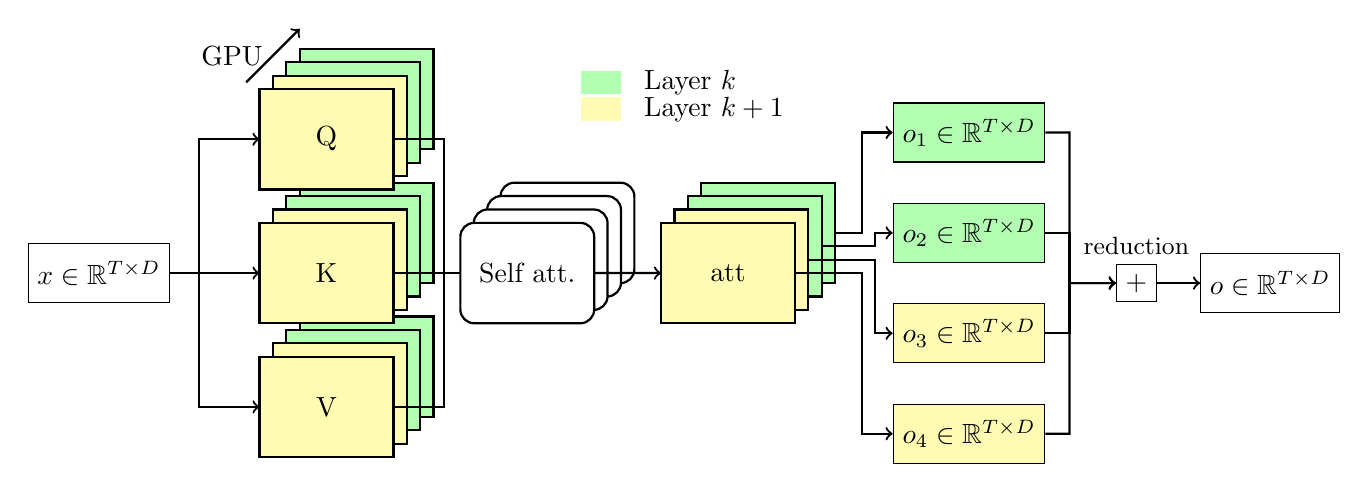
\begin{tikzpicture}[scale=0.85,
        box/.style={draw, rectangle, minimum width=1.5cm, minimum height=0.75cm},
        reducebox/.style={draw, rectangle, minimum width=0.3cm, minimum height=0.3cm},
        arrow/.style={->, thick},
        line/.style={-, thick},
    ]
    % Add diagonal GPU arrow
    \draw[->, thick] (2.2, 3) -- node[above, left] {GPU} (3, 3.8);
    
    % Add color legend
    \node[rectangle, fill=green!30, minimum width=0.5cm, minimum height=0.3cm] at (7.5, 3) {};
    \node[right] at (8, 3) {Layer $k$};
    \node[rectangle, fill=yellow!30, minimum width=0.5cm, minimum height=0.3cm] at (7.5, 2.6) {};
    \node[right] at (8, 2.6) {Layer $k+1$};
    
    \node[box] (input) at (0, 0.15) {$x\in\mathbb{R}^{T\times D}$};
    \stackedrectangles[3,-2]{V}{green!30}{yellow!30}{V};
    \stackedrectangles[3,0]{K}{green!30}{yellow!30}{K};
    \stackedrectangles[3,2]{Q}{green!30}{yellow!30}{Q};
    \draw[arrow] (input) -- +(1.5,0) |- (Q-E4left);
    \draw[arrow] (input) -- +(1.5,0) |- (K-E4left);
    \draw[arrow] (input) -- +(1.5,0) |- (V-E4left);
    \stackedroundedrectangles[6, 0]{mha}{white}{white}{Self att.};
    \draw[line] (Q-E4right) -- +(0.75, 0) |- (mha-E4left);
    \draw[line] (K-E4right) -- +(0.75, 0) |- (mha-E4left);
    \draw[line] (V-E4right) -- +(0.75, 0) |- (mha-E4left);
    \stackedrectangles[9, 0]{att}{green!30}{yellow!30}{att};
    \draw[arrow] (mha-E4right) -- (att-E4left);
    \node[box, fill=green!30] (o1) at (13, 2.25) {$o_1\in\mathbb{R}^{T\times D}$};
    \node[box, fill=green!30] (o2) at (13, 0.75) {$o_2\in\mathbb{R}^{T\times D}$};
    \node[box, fill=yellow!30] (o3) at (13, -0.75) {$o_3\in\mathbb{R}^{T\times D}$};
    \node[box, fill=yellow!30] (o4) at (13, -2.25) {$o_4\in\mathbb{R}^{T\times D}$};
    \draw[arrow] (att-E4right) -- +(1, 0) |- (o4);
    \draw[arrow] (att-E3right) -- +(1, 0) |- (o3);
    \draw[arrow] (att-E2right) -- +(0.8, 0) |- (o2);
    \draw[arrow] (att-E1right) -- +(0.4, 0) |- (o1);
    
    % Add allreduce box
    \node[reducebox] (allreduce) at (15.5, 0) {$+$};
    \node[above] at (allreduce.north) {\small reduction};
    
    % Add arrows from o boxes to allreduce
    \draw[arrow] (o1) -- +(1.5,0) |- (allreduce);
    \draw[arrow] (o2) -- +(1.5,0) |- (allreduce);
    \draw[arrow] (o3) -- +(1.5,0) |- (allreduce);
    \draw[arrow] (o4) -- +(1.5,0) |- (allreduce);
    
    % Add final output box
    \node[box] (output) at (17.5, 0) {$o\in\mathbb{R}^{T\times D}$};
    \draw[arrow] (allreduce) -- (output);
\end{tikzpicture}
\caption{\label{fig:tplpcombo} Generalization of Layer Parallelism and Tensor Parallelism. In this case, the figure shows the case for 4 GPUs and 2 layers. The stacked layers represent the tensor parallelism, and the colors indicate the processing of different previously contiguous layers. LP builds on top of TP by assigning the heads from consecutive layers into different GPUs. If there are more GPUs than layers, then each layer will be accelerated using TP, and $Q,K,V\text{ and }att \in\mathbb{R}^{T\times \frac{2D}{g}}$, where $D$ is the feature dimension and $g$ is the total number of GPUs.}
\end{figure*}

\end{document}